%******************************FORMATIERUNG****************************************
\documentclass[a4paper, 12pt]{article}
\usepackage{scrpage2}
\usepackage{todonotes}
\pagestyle{scrheadings}
\clearscrheadfoot
\setheadsepline{.5pt}
\setfootsepline{.5pt}
\automark[section]{chapter}
\ihead{\headmark}
%\ihead{\headmark}
\ohead{\pagemark}
\usepackage[ngerman]{babel}
\usepackage[utf8]{inputenc}
\usepackage{graphicx}
\usepackage[space]{grffile}
 \usepackage{setspace}
\usepackage[T1]{fontenc}
\newcommand{\changefont}[3]{
\fontfamily{#1} \fontseries{#2} \fontshape{#3} \selectfont}
\usepackage{datetime}
\newdateformat{monthyeardate}{%
  \monthname[\THEMONTH] \THEYEAR}
\usepackage{geometry}
\geometry{verbose,a4paper,tmargin=30mm,bmargin=30mm,lmargin=35mm,rmargin=25mm}
\usepackage[numbers,square]{natbib}
\usepackage[breaklinks=true]{hyperref}
 \usepackage{algorithmicx}
 \usepackage[ruled]{algorithm}
\usepackage{algpseudocode}
\setlength{\parindent}{0pt} 
\usepackage{color}
\definecolor{myColor}{rgb}{0.8,0.8,0.8}

%*****************************ENDE FORMATIERUNG****************************************

\begin{document}
\linespread{1.2}
\changefont{ppl}{m}{n}

%INHALTSVERZEICHNIS
%\pagenumbering{arabic}
%\tableofcontents
\newpage

\thispagestyle{empty}
\begin{center}
			
\includegraphics[width=5cm]{Bilder/logo_TH}\\[12ex]
			{\Huge\textbf{Projektdokumentation}}\\[8ex]
			\rule{.8\textwidth}{.2pt}
			{\Large\\[1ex] \textbf{MArC}}\\
			{\textbf{M}ixed Reality \textbf{Ar}chitecture \textbf{C}omposer}\\
			\rule{.8\textwidth}{.2pt}\\[10ex]
			von\\[2ex]
			\begin{tabular}{ll}
			Laura Anger &(Matrikelnr. 11086356)\\ 
			Vera Brockmeyer &(Matrikelnr. 11077082)\\
			Paul Berning &(Matrikelnr. xxxxxxxxxx)\\
			Lukas Kolhagen &(Matrikelnr. 11084355)\\
			\end{tabular}\\[10ex]
			Durchgeführt im\\ \textbf{Master Medientechnologie}\\
			im \textbf{SS 2016} und \textbf{WS 2016/17}\\			
			\end{center}
			\vfill
			\begin{flushleft}
			{\bf Betreuer:}\\
			Prof. Dr. Stefan Michael Grünvogel\\
			Institut für Medien- und Phototechnik
			\end{flushleft}
	\newpage
	\tableofcontents
	\newpage

\section{Einleitung}
Virtuelle und erweiterte Realität ist bereits seit einiger Zeit in aller Munde. Mit dem Erscheinen von Oculus Rift, HTC Vive und anderen Virtual-Reality-Headsets rückt eine neue Art der Immersion beim Genuss von Videospielen in greifbare Nähe.\\
Wenn es jedoch um die Nutzung dieser Technologien zur Effizienzsteigerung in professionellen Umgebungen geht, so sind verfügbare Anwendungen bisher noch Mangelware.
Die Entwicklung des AR2-Composer, einem Virtual-Reality-System für die architektonische Planung bei Siedlungsbauten, soll dies ändern.
\subsection{Anwendungskontext}
Die frühe Konzeptionierung zur Erschließung von Wohngebieten findet heute in Architekturbüros meist noch so statt wie vor {\color{red}??} Jahren. Dazu werden simple Modelle aus leicht zu verarbeitenden Materialien -- wie etwa Styropor -- erstellt und als Platzhalter für die zu planenden Gebäude bei dem Entwurf verwendet.\\
Diese Herangehensweise macht Änderungen an den Gebäuden aufwendig und führt zu dem Umstand, dass ein bestimmter Zustand der Planung nur umständlich wiederhergestellt werden kann -- zum Beispiel durch Fotografieren und späteren manuellen Wiederaufbau.
\subsection{Projektziel}
\section{Grundlagen und Stand der Wissenschaft} \label{sec:grundlagen}
\todo[inline, color=red]{Paul}
\todo[inline, color=green]{Vera}
Im folgenden werden die Grundlagen und der Stand-der-Wissenschaft von allen Teilbereichen des \textit{MArC} Systems erläutert. Es werden Veröffentlichungen von ähnlichen Architektur VR-Anwendungen, haptischen Interaktionsmethoden sowie Handtracking Methoden erläutert. Fortlaufend wird auf die Grundlagen der Netzwerktechnologie und den bekanntesten Bedienkonzepten in VR- Umgebungen eingegangen. Zuletzt werden die wichtigsten Methoden zu der Marker-Verfolgung zusammengefasst.
\subsection{Architektur von Virtual-Reality-Anwendungen}\label{sec:ArchitekturAnwendungen}\todo[inline, color=green]{Lukas}
\todo[inline, color=red]{Paul}
Bei der Entwicklung von Virtual Reality (VR) Anwendungen gibt es zwei entscheidende Unterschiede im Vergleich zu herkömmlichen Software-Anwendungen~\cite{bryson1995approaches}:
\begin{itemize}
	\item Die virtuelle Umgebung und das damit verbundene Interface sollten auf die vorliegende Aufgabe zugeschnitten werden und
	\item Spezielle Anforderungen an die Performanz der Anwendung müssen erfüllt sein, damit die virtuelle Realität erfolgreich präsentiert werden kann.
\end{itemize}

Als grundsätzlich unterschiedliche Architekturen bei der Entwicklung von VR-An\-wen\-dung\-en kann nach Hardware-Plattformen unterschieden werden:
\begin{description}
	\item[Desktop-VR-Applikationen:] Hierbei handelt es sich um die leistungsstärksten VR-Applikationen, die potente Computer-Hardware häufig mit Head-Mounted-Displays wie etwa \textit{Oculus Rift} oder \textit{HTC Vive} verwenden.
	\item[Mobile-VR-Applikationen:] Mobile Anwendungen vereinen häufig (jedoch nicht immer) alle notwendige Hardware in einem Gerät, wie etwa einem Smartphone oder Tablet-Computer.\\ Beispiele für mobile VR-Anwendungen sind \textit{Samsung GearVR}~\cite{website:gearVRpressRelease} und \textit{Google Cardboard}~\cite{website:googleCardboard}. Im Falle von \textit{Samsung GearVR} und \textit{Google Cardboard} wird zusätzlich eine Haltevorrichtung für das verwendete Gerät eingesetzt, die bei \textit{GearVR} auch als Controller fungiert und durch ein integriertes Linsensystem das Sichtfeld des Benutzers erhöht.
	\item[Web-VR-Applikationen:] Anwendungen für das Web wie etwa WebVR~\cite{website:webVR} erlauben den Zugriff auf Virtual-Reality-Geräte wie Head-Mounted-Displays durch einen Browser. Auf diese Weise können Web-Inhalte mit VR-Hardware konsumiert werden.
\end{description}

Die Entscheidung, für das vorliegende Projekt auf eine Desktop-VR-Anwendung zu setzen, wurde getroffen, weil mobile und Web-VR-Applikationen die folgenden, vom Projektteam als unverzichtbar eingestuften Voraussetzungen nicht erfüllen konnten.
\begin{itemize}
	\item Es sollte möglich sein, die in Abschnitt \ref{sec:HandtrackingAnwendungen} beschriebenen Handtracking Interaktionsmethoden für die Verwendung von haptischen Würfel-Markern zu verwenden.
	\item Außerdem sollte die verwendete Architektur ein zuverlässiges Echtzeit-Tracking mit geringer Latenz von mindestens einem Dutzend Markern erlauben, wie es in Abschnitt \ref{sec:MarkerTracking} beschrieben wird.
	\item Und schließlich sollte \emph{MArC} die Basis bereitstellen, um später auch mit mehreren Benutzern verwendet werden zu können.
\end{itemize}

\subsection{Haptische Interaktionsmethoden in VR Umgebungen}\label{sec:HaptikAnwendungen}\todo[inline, color=green]{Laura}
\todo[inline, color=red]{Paul}
Um das Eintauchen in die virtuelle Welt zu erleichtern, kann es bei manchen VR-Anwendungen sinnvoll sein, dem Benutzer eine Form von haptischem Feedback zu geben. Die meisten solcher Systeme mit haptischen Feedback haben ihren Ansatzpunkt an den Fingern, oder genauer gesagt an den Fingerspitzen. Es gibt aber auch Systeme die mehrere Parts des Körpers oder sogar den ganzen Körper mit einbeziehen.\\
Man unterscheidet zwischen \textit{Active Feedback Devices} und \textit{Passive Feedback Devices}. Während die aktive Variante dynamisch veränderliche Kräfte erzeugt, die dem Benutzer entgegenwirken, werden die passiven Varianten immer nur durch den Benutzer selber bewegt \cite{Haptic}.\\
Um eine genauere Unterteilung vorzunehmen, kann man die verschiedenen Systeme zudem nach den einzelnen haptischen Wahrnehmungen unterteilen. Eine mögliche Aufteilung ist im Folgenden zu sehen.

\begin{description}
	\item[Force Feedback Systeme:] Ausübung eines Kraftvektors auf eine Körperstelle des Benutzers, um seine Bewegung zu erschweren oder aktiv eine Bewegung zu erzwingen. %Ein Beispiel hierfür ist das Exoskelett für die Hand von \textit{Dexta Robotics} \cite{Gu:2016:DIL:2858036.2858487}.
	\item[Tactile Feedback Systeme:] Stimulation der Berührungsempfindung der Haut. Im Allgemeinen wird ein variabler Druck auf eine Hautstelle ausgeübt, welcher nicht direkt von der Bewegung des Körperteils abhängig ist.
	\item[Greifen:] Kann als Kombination der beiden vorangegangen Ansätze angesehen werden. Befindet sich ein virtueller Gegenstand in der Hand so soll hierbei verhindert werden können, dass der Benutzer seine Hand schließt. 
	\item[Proprioceptive Feedback Systeme:] Im Gegensatz zu den \textit{Tactile Feedback Systems} spürt der Anwender nicht über seine Haut, sondern über Gelenke bzw. Muskeln. 
\end{description}

Bei den oben aufgelisteten Formen von haptischer Interaktion wird davon ausgegangen, dass der Gegenstand um den es geht, rein virtueller Natur ist. Eine Besonderheit an \textit{MArC} ist, dass es sich um reale Objekte (vgl. Abschnitt~\ref{sec:WürfelMarker}) handelt, an deren Position virtuelle Objekte gerendert werden können. In diesem dog \textit{Mixed-Reality}-System hat der Benutzer also einen realen haptischen Eindruck. Der reale Würfel dient somit als Anfasser und bietet die Möglichkeit das virtuelle Objekt, was durchaus größer (oder auch flacher) als sein reales Pendant sein kann, zu transformieren. 

%In manchen Fällen kann es schwierig sein eine eindeutige Zuordnung des Systems zu einer der Kategorien zu finden.


\subsection{Handtracking}\label{sec:HandtrackingAnwendungen}\todo[inline, color = green]{Paul}
\todo[inline, color=blue]{Lukas}
 -Handtracking ist mittels verschiedener Trackingsysteme möglich. Alle Systeme haben hierbei ihre Vor- und Nachteile. \\
 -Beispielsweise ist es möglich, die Bewegungen der Hand mittels eines Datenhandschuhs zu erfassen. Dies ist ein mit Sensoren ausgestatteter Handschuh, den der Nutzer an den Händen trägt. Eine Möglichkeit die Fingerbewegung mit einem Datenhandschuh zu erfassen sind Biegesensoren. Hierbei handelt es sich je nach Bauart um Glasfasern, die an den Fingern entlang laufen. Wird ein Finger gebogen, wird ein Licht welches durch die gebogene Glasfaser läuft, leicht abgeschwächt. Hierdurch ist eine Biegung erkennbar. Dieses System ist ebenfalls mittels gefärbter Flüssigkeit innerhalb kleiner Röhrchen möglich. Auch hier werden bei Bewegung weniger Partikel durchgelassen.\\
 -Eine weitere Möglichkeit ist das Exosklett. Hierbei wird eine Mechanik an dem Handschuh angebracht, mittels welcher Bewegungen auf Sensoren übertragen werden. Datenhandschuhe sind für den Nutzer einschränkend und aus Hygienischen Gründen nicht die Beste Wahl zum Handtracking.\\
 -Eine bessere Möglichkeit ist das optische Tracking der Hande. Systeme wie der \textit{Leap Motion Controller} erfassen mit Kameras die Shilouette der Hände und rechnen aus den stereoskopischen Bildinformationen die Winkel und Positionen der verschiednen Fingerglieder aus.\\
 -Dieses System ist einfach zu benutzen, sobald der Nutzer seine Hand in den getrackten Bereich hält, werden diese erkannt.\\
 -Typisch für optische Systeme ist jedoch das Problem der Verdeckung. Wird die Hand aus einer bestimmten Richtung durch Kameras gefilmt, kann es passieren, dass einige Finger andere überdecken. Teilweise kann dann nicht exakt unterschieden werden, welches Fingerlied zu welchem Finger oder Teil der Hand gehört. Dies wirkt sich bei der Benutzung in einem "hüpfenden" Verhalten oder unmenschlich verrenkter Finger aus.
\subsection{ISO/OSI-7-Schichtenmodell}\label{sec:Netzwerk}\todo[inline, color=green]{Laura}
\todo[inline, color=red]{Paul}
Um die Kommunikation zwischen unterschiedlichsten technischen Systemen zu ermöglichen und zu vereinheitlichen dient das \textit{ISO/OSI-7-Schichtenmodell} \cite{ITU}, welches in Tabelle~\ref{tab:Schichtenmodell} schematisch dargestellt ist. Um die Weiterentwicklung von Kommunikationsmodellen möglichst barrierefrei zu gestalten, sind in dem Modell sieben aufeinanderfolgende Schichten definiert worden, die für einen jeweils klar eingegrenzten Teilbereich der Kommunikation zuständig sind. Die Netzprotokolle, die in einer Schicht zum Einsatz kommen, müssen einheitliche Schnittstellen aufweisen, um einen reibungslosen Austausch zu gewährleisten. Entsprechende Beispiele sind der rechten Spalte von Tabelle~\ref{tab:Schichtenmodell} zu entnehmen.\\

\begin{table}
	\centering
	\renewcommand{\arraystretch}{1.4}
	\begin{tabular}{|c|c|c|}
		\hline
		\Absatzbox{}
		\textbf{Nr.} & \textbf{Schicht}&\textbf{Beispiel}\\
		\hline
		7 & Anwendung &  HTTP, SMTP, FTP, DNS\\
		\hline
		6 & Darstellung & HTTP, SMTP, FTP, NNTP, NetBIOS\\
		\hline
		5 & Sitzung& HTTP, SMTP, FTP, NNTP, NetBIOS, TFTP\\
		\hline
		4 & Transport & TCP, UDP, SPX, NetBEUI\\
		\hline
		3 & Vermittlung& IP IPX\\
		\hline
		2 & Sicherung & Ethernet, ATM, FDDI, TR\\
		\hline
		1 & Bitübertragung & Manchester, 10B5T, Trellis\\
		\hline
	\end{tabular}
	\caption{ISO-/OSI-7-Schichtenmodell}
	\label{tab:Schichtenmodell}
\end{table}

Während die Schichten 1--4 als transportorientierte Schichten einzustufen sind, können die verbleibenden Schichten 5--7 als anwendungsorientiert angesehen werden. Da der Austausch von Daten für die Umsetzung von \textit{MArC} im Vordergrund steht, wird im Folgenden besonders auf die vierte Schicht eingegangen. Dabei werden die beiden Übertragungsprotokolle \textit{Transmission Control Protocol} (TCP) und \textit{User Datagram Protocol} (UDP) vorgestellt. Auf die Aufführung weiterer Übertragungsprotokolle wird bewusst verzichtet.\\
Die Transportschicht stellt eine logische Ende-zu-Ende-Verbindungen dar und dient als Bindeglied zwischen den transportorientierten und anwendungsorientierten Schichten \cite{ITU}.

\begin{description}
\item[TCP:] Dieses Transportprotokoll ist verbindungsorientiert und paketvermittelt. Genaue Details können in dem Standard RFC 793 \citep{rfc793} von 1981 in Erfahrung gebracht werden.

\item[UDP:] Dieses Transportprotokoll wurde aus der Notwendigkeit heraus entwickelt, für die Übertragung von Sprache auf ein, im Gegensatz zur TCP, simpleres Protokoll zurückgreifen zu können. Genaue Details können in dem Standard RFC 768 \citep{rfc768} von 1981 in Erfahrung gebracht werden.
\end{description}

Ein wichtiger Unterschied zwischen den beiden Transportprotokollen ist, dass die Übertragung per TCP im Vergleich zu UDP sicherstellt, dass gesendete Daten korrekt übertragen und empfangen werden. Dies geschieht dadurch, dass in einem TCP-Socket-Netzwerk Fehlererkennungs- und Korrekturmechanismen enthalten sind, die fehlerhafte Übertragungen der darunterliegenden Internet Protocol (IP) Schicht ausgleichen, also entweder korrigieren oder dafür sorgen, dass fehlerhafte Daten erneut übertragen werden.

\subsection{Bedienkonzepte in VR-Umgebungen}\label{sec:MenüAnwendungen}\todo[inline, color=green]{Lukas}
\todo[inline, color=red]{Paul}
Die Bedienung eines Systems~--~vor allem die Dateneingabe und Objektmanipulation~--~in einer Virtual Reality (VR) Umgebung unterscheidet sich stark von der konventionellen Bedienung mit Maus und Tastatur \cite{chu1997multi}. Das Hauptziel einer VR-Umgebung ist die sog. Immersion, also das "`Eintauchen"' des Benutzers in die virtuelle Welt. Ein Teil zur Erreichung dieses Ziels sind Methoden, mit denen der Benutzer mit der virtuellen Welt~--~möglichst intuitiv~--~interagieren kann.

Nach~\cite{sherman2002understanding} gibt es vier unterschiedliche Manipulationsmethoden für VR-An\-wen\-dung\-en:
\begin{description}
	\item[Direct User Control:] Der Benutzer interagiert mit Objekten in der virtuellen Welt so, wie dieser es auch in der realen Welt tun würde. Ein Beispiel hierfür ist eine Geste wie das Schließen der Hand zu einer Faust, um einen Gegenstand in der virtuellen Welt "`anzufassen"', sodass dieses Objekt anschließend der Bewegung der Hand folgt.
	\item[Physical Control:] Manipulationen in der virtuellen Welt geschehen durch die Interaktion des Benutzers mit einem realen Gegenstand. Ein solcher Gegenstand kann beispielsweise ein Lenkrad oder ein Joystick sein.
	\item[Virtual Controls:] Bei \emph{Virtual Controls} handelt es sich nicht direkt um eine Manipulationsmethode, viel mehr beschreibt der Begriff die in der virtuellen Welt vorhandenen Interaktionsmodule, wie etwa Buttons, die gedrückt werden können. Um tatsächlich zu interagieren muss der Benutzer eine der drei anderen Manipulationsmethoden verwenden.
	\item[Agent Controls:] Der Benutzer interagiert mit der virtuellen Welt über einen "`intelligenten Mittelsmann"'. Dieser Mittelsmann kann eine Person oder ein vom Computer kontrolliertes Wesen sein.
\end{description}
In den Abschnitten~\ref{sec:kontextMenu}, \ref{sec:markerHandles} und \ref{sec:TableMenü} wird auf die in \emph{MArC} verwendeten Interaktions- und Manipulationsmethoden eingegangen.

\subsection{Marker Verfolgung} \label{sec:MarkerTracking}\todo[inline, color=green]{Vera}
\todo[inline, color=red]{Paul}
In einer VR- oder AR-Umgebung ist zur interaktiven Positionierung eines 3D Objektes die präzise Bestimmung der Orientierung und Position im 3D-Zielraum notwendig. Zur Lösung dieses Problems muss zunächst ein physisches Objekt in der realen Welt erkannt, zugeordnet und verfolgt werden. Demzufolge ist es notwendig, dieses physische Objekt mit einer Videokamera aufzunehmen. In den resultierenden Bildsequenzen werden die physischen Objekte anhand von festgelegten Merkmalen erkannt. Diese Merkmale können sowohl natürlicher Art sein oder in Form von künstlich erstellten Codes festgelegt sein. Ein Objekttracking mit natürlichen Merkmalen wird in der Literatur auch als \textit{Markerless Tracking} bezeichnet, während die Verwendung von Codes, beziehungsweise Bildmarken, als \textit{Markerbased Tracking} bekannt ist.

Natürliche Merkmale zur Identifizierung der Objekte sind Textureigenschaften, Kanteninformationen oder sogenannte Keypoints. Eine der robustesten und simpelsten Methoden ist die Verwendung von Keypoints \cite{article:MarkerLessBarandiaran2010}\cite{article:MarkerLessWagner:}\cite{article:MarkerLessComport}\cite{article:MarkerLessLowe}, die sowohl in der Ausgangs- als auch in der Kamerawelt bekannt beziehungsweise ermittelbar sind. Diese werden mit Hilfe einer Homographie zur Übereinstimmung gebracht. Daraus resultiert die notwendige Transformation zwischen den Welten (siehe Kapitel \ref{sec:calib}). Ein bedeutender Nachteil der Verwendung von Keypoints oder Texturbasierten Verfahren ist, dass sie nur für Objekte mit einem hohen Grad an Texturmerkmalen und großen Gradientenbeträgen geeignet sind. Aus diesem Grund wurden auch Verfahren \cite{article:MarkerLessStrucktHinterstoisser}\cite{article:MarkerLessStrucktDamen}\cite{article:MarkerLessStrucktPark} entwickelt die sich speziell für texturarme Objekte eignen, wie etwa die in \textit{MArC} verwendeten grünen Rechtecken der Würfel Marker (siehe Kapitel \ref{sec:WürfelMarker}). Andere Autoren verwenden sehr rechenintensive Kantenerkennungsalgorithmen, wie den \textit{Moving Edges Algorithm} \cite{article:MarkerLessEdgeMarchand}. Eine weitere Weiterentwicklung der Kantenbasierten Methoden ist das Modelbased Tracking bei dem die detektierten Kanten eines möglichen Kandidaten mit den 3D-Kantenmodellen des zu verfolgenden Objektes abgeglichen wird \cite{article:MarkerLessModellVacchetti}\cite{article:MarkerLessEdgeAlvarez}\cite{article:MarkerLessEdgeWu}\cite{article:MarkerLessBlasko}.

Im Gegensatz zu dem \textit{Markerbased Tracking} benötigt das \textit{Markerless Tracking} keine Veränderung oder Anpassung der realen Welt. Doch die Parameter, welche den Tracking-Algorithmus beeinflussen, können nicht ohne Weiteres kontrolliert werden \cite{article:MarkerLessBarandiaran2010}. Dennoch ist das \textit{Markerless Tracking} von Objekten sehr rechenaufwändig und eine eindeutige Zuordnung beziehungsweise Identifikation von ähnlichen oder gleichförmigen Objekten, wie zum Beispiel den Würfel Marker, ist sehr aufwändig und nahezu unmöglich. Aus diesem Grund ist es für ein System wie \textit{MArC} zum derzeitigem Zeitpunkt sinnvoller die Würfel Marker mit codebasierten Mustern zu erweitern, die auch nach längerer Verdeckung eine eindeutige Zuordnung von Würfel Marker ermöglichen. In Abbildung \ref{fig:BinMarker} sind vielfältige Beispiele von binären Codes zu sehen, die zum Marker Tracking verwendet werden. Für \textit{MArC} sind vor allem rechteckige binäre Muster vorteilhaft, da aus dem äußeren vier Ecken auch die Orientierung des Würfel Markers im Raum abgeleitet werden kann. Während der Inhalt des Muster zur eindeutigen Identifizierung des Würfels beiträgt. 

Bekannte markerbasierte Verfahren mit rechteckigen binären Mustern sind das bekannte \textit{QR}-Verfahren, \textit{ARToolKit}\cite{article:MarkerARTOOL}, \textit{ARToolKit Plus}\cite{article:MarkerARTOOL2}, \textit{ARTag} \cite{article:MarkerARTag}, \textit{BinARyID} \cite{article:MarkerBinAR} und \textit{ArUco}\cite{article:Aruco2014}. Wie in Abbildung \ref{fig:BinMarker} zu sehen ist, sind bis auf \textit{BinARyID} und \textit{ArUco} alle Muster sehr detailreich und komplex. Diese Eigenschaft ist auf die höhere Bitanzahl der Codes zurückzuführen macht die Erkennung in Aufnahmen aus größerem Abstand und möglicher mit Bewegungsunschärfe ungleich schwerer. Es kommt unter diesen Umständen häufiger zu Fehlinterpretationen und Ausfällen. Gerade in einem System wie \textit{MArC} tritt Bewegungsunschärfe sehr häufig auf, da die Würfel Marker regelmäßig bewegt werden. Auch der verhältnismäßig große Abstand der Kamera zu den Würfel-Markern lässt die Markermuster im Kamerabild relativ klein werden und somit wirkt sich die Bewegungsunschärfe noch deutlicher auf die feinen Codemuster aus. Darum eigen sich hier vor allem Muster mit geringer Bitanzahl und groben Mustern, wie zum Beispiel \textit{ArUco} Marker mit einer $16$ bit Codierung. Diese Marker Bibliothek ist ein \textit{OpenCV}-Modul (siehe Kapitel \ref{sec:OpenCV}), welche alle notwendigen Funktionalitäten und Ressourcen für das Tracking und die Orientierungsbestimmung der physische Objekt enthält. Ein weiterer großer Vorteil dieser Bibliothek ist, dass die Bitgröße und maximale Anzahl der Identitäten explizit ausgewählt werden kann.


\begin{figure}[H] 
	\center 
	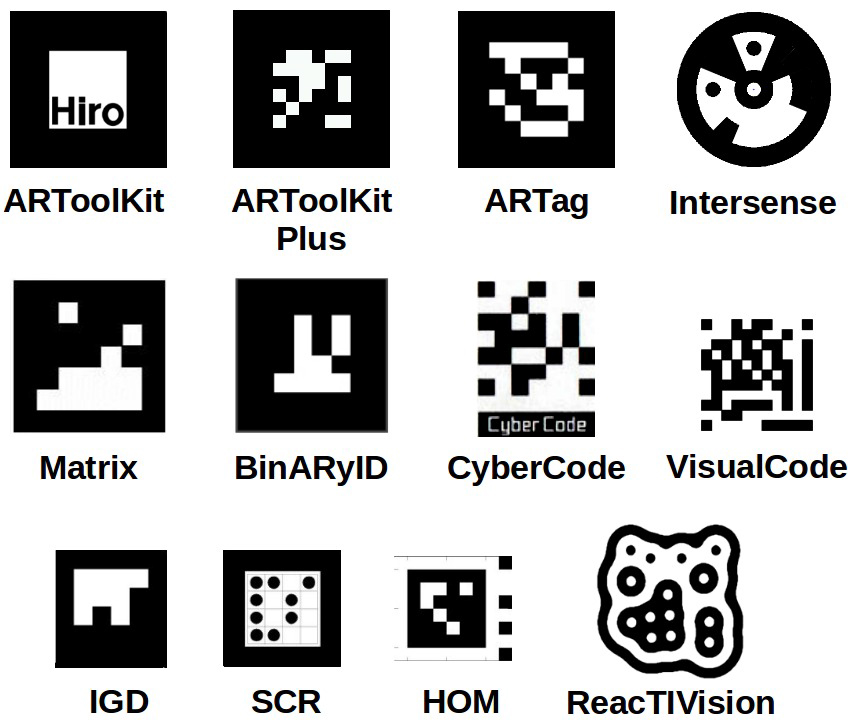
\includegraphics[width=8cm]{Bilder/BinMuster.jpg}			
	\caption{Diverse Binäre Muster die als Code für Markerbasiertes Tracking verwendet werden. Quelle: \cite{article:Aruco2014}}
	\label{fig:BinMarker}
\end{figure}

\newpage
\section{Materialien}\label{sec:Materialien}
In den nachfolgenden Abschnitten, werden Werkzeuge und Hilfsmittel beschrieben, die für die Fertigstellung des Projekts vonnöten waren.\\ Des weiteren werden auch Komponenten vorgestellt, die während der Projektlaufzeit erstellt wurden, wie etwa die Würfel-Marker (s. Abb.~\ref{fig:marker}).

\subsection{Hardware}
Zur Ausführung der \emph{MArC}-Software sind diverse Hardware-Komponenten Voraussetzung. Diese Komponenten werden nachfolgend beschrieben und deren Kontext im System näher erläutert.
\subsubsection{Computer zur Ausführung der Unity-Simulation}\label{sec:UnityComp}\todo[inline, color=green] {Lukas}
Die Anwendung, welche aus Unity \cite{website:Unity} heraus erstellt wurde, benötigt einen Host-Computer, welcher sowohl mit dem HTC Vive Head-Mounted Display kompatibel, als auch leistungsstark genug sein muss, um das Rendering der Simulation mit ausreichend hoher Bildrate ausführen zu können.

Für das vorliegende Projekt wurde seitens der Technischen Hochschule Köln ein Computer zur Verfügung gestellt. Die technischen Daten des Geräts sind in Tabelle~\ref{tab:UnityCompParam} aufgeführt.

\begin{table}
	\centering
	\begin{tabular}{|l|l|}
		\hline
		\Absatzbox{}
		\textbf{CGPC6}& \textbf{Beschreibung} \\
		\hline
		Prozessor & Intel Core i7 6700 CPU @ $4\times3.4-4.0$\,GHz \\
		\hline
		Arbeitsspeicher & $16$\,GB \\
 		\hline 
		Grafikkarte & NVIDIA GeForce GTX 980\\
		\hline
		Betriebssystem & Windows 10 Education 64 bit \\
		\hline
		Schnittstellen & $2\times$ USB 3.0, $5\times$ USB 2.0, $1\times $ HDMI\\
		\hline
	\end{tabular}
	\caption{Übersicht der technischen Daten des Computers für die Unity-Simulation.}
	\label{tab:UnityCompParam}
\end{table}

Die Hard- und Software-Voraussetzungen für die Ausführung der Unity-Anwendung in Verbindung mit der HTC Vive, welche in Tabelle~\ref{tab:viveReq} aufgelistet sind, werden von dem verwendeten Computer übertroffen.

\begin{table}
	\centering
	\begin{tabular}{|l|l|}
		\hline
		\Absatzbox{}
		\textbf{HTC Vive}& \textbf{Systemvoraussetzungen} \\
		\hline
		Prozessor & mindestens Intel Core i5-4590 oder AMD FX 8350\\
		\hline
		Grafikkarte & mindestens NVIDIA GeForce™ GTX 1060\\
		&oder AMD Radeon™ RX 480\\
		\hline
		Arbeitsspeicher & mindestens $4\,GB$\\		
		\hline
		Videoausgang & $1\times$ HDMI 1.4-Anschluss oder DisplayPort 1.2\\
		\hline
		USB & $1\times$ USB 2.0-Anschluss\\
		\hline
		Betriebssystem & Windows 7 SP1, Windows 8.1 oder Windows 10\\
		\hline
	\end{tabular}
	\caption{HTC Vive Systemvoraussetzungen. \cite{website:HTC_Vive_Ready}}
	\label{tab:viveReq}
\end{table}

\subsubsection{Computer zur Ausführung der Tracking-Anwendung}\label{sec:TrackingComp}\todo[inline, color=green]{Vera}

Auf Grund der begrenzten Bandbreite einer USB-Karte ist es zwingend notwendig einen weiteren Rechner an das Gesamtsystem zu koppeln, welcher ausschließlich für die Ansteuerung der uEye-Kamera und die Berechnungen des Tracking-Algorithmus zuständig ist. 
An den Computer zur Ausführung der VR Umgebung sind gezwungenermaßen viele externe USB Komponenten, wie zum Beispiel die \textit{Leap Motion} und die \textit{HTC Vive}, angeschlossen. Dies führt zu einer hohen Auslastung der Bandbreite der USB-Karte und auf Grund dessen ist es nicht mehr möglich die uEye-Kamera mit der notwendigen maximalen Framerate zu betreiben. Somit wird für ein flüssiges und real-time fähiges Tracking der \textit{Acer E5-571G-795A} mit den Eigenschaften aus Tabelle \ref{tab:TrackingCompParam} verwendet.

\begin{table}
	\centering
	\begin{tabular}{|l|l|}
		\hline
		\Absatzbox{}
		\textbf{Acer E5-571G-795A}& \textbf{Beschreibung} \\
		\hline
		Prozessor & Intel Core i7-5500U CPU @ $2\times 2.4-3.0$\,GHz\\
		\hline
		Arbeitsspeicher & $8.0$\,GB \\
		\hline 
		Grafikkarte & NVIDIA GeForce 840M\\
		\hline
		Betriebssystem & Windows 10 Home, 64 bit \\
		\hline
		Schnittstellen & $2\times$ USB 2.0, $1\times$ RJ45-Netzwerkanschluss\\
		\hline
	\end{tabular}
	\caption{Auszug aus dem technischen Datenblatt des \textit{Acer E5-571G-795A}.}
	\label{tab:TrackingCompParam}
\end{table}


\subsubsection{HTC Vive}\label{sec:Vive} \todo[inline, color=green]{Laura}
Bei der \textit{HTC Vive} handelt es sich um ein Head-Mounted Display, welches von \textit{HTC} in Kooperation mit \textit{Valve}~\cite{website:Valve} produziert wird. Vorgestellt wurde dieses am 1. März 2015 im Vorfeld des \textit{Mobile World Congress}~\cite{website:mobileworldcongress}.\\
Die Auflösung des Displays beträgt insgesamt $2160\times1200$ Pixel, was $1080\times1200$ Pixeln pro Auge enstpricht. Die Brille bietet ein Sichtfeld von bis zu $110^\circ$ bei einer Bildwiederholrate von $90\,Hz$ \cite{website:HTC_Vive}. Alle technischen Systemvoraussetzungen können in Tabelle \ref{tab:viveReq} eingesehen werden. \\
Zur Positionsbestimmung im Raum wird die Lighthousetechnologie von \textit{Valve} genutzt. Zusätzlich sind neben einem Gyrosensor auch ein Beschleunigungsmesser und ein Laser-Positionsmesser verbaut. Mittels speziellen Game-Controllern wird eine Interaktion mit virtuellen Objekten ermöglicht.

\subsubsection{IDS uEye 164LE-C}\label{sec:uEye} \todo[inline, color=green] {Vera}
Die Kamera \textit{uEye 164LE-C} wurde vom Hersteller \textit{IDS Imaging Development Systems} entwickelt. Sie hat eine Bildauflösung von $1280 \times 1024$ Pixel und ermöglicht Live-Video-Aufnahmen im RGB Farbmodus mit maximal $25$ fps. Der integrierte CMOS Bildsensor wird im Rolling Shutter Modus betrieben und ermöglicht Belichtungszeiten von $37\mu$s bis $10$s. Weiterführend kann sie universell mit allen gängigen Computern oder Systemen via USB 2.0 Schnittstelle verbunden werden \cite{website:UEyeTechSpec}.\\

Die erforderliche Ansteuerung der \textit{uEye 164LE-C} erfolgt mit Hilfe der bereit gestellten \textit{IDS Software Suite}. In diese Suite ist die \textit{uEye-API} integriert, welche die Entwicklung von eigenen Programmen unter den Betriebsystemen \textit{Windows} und \textit{Linux} mit den Programmiersprachen \textit{C}$++$, \textit{.NET}, \textit{C$\#$} oder \textit{C} ermöglicht \cite{website:IDSSuite}. Für das Tracking der Marker in \textit{MArC} wurde eine eigene Schnittstelle in \textit{C}$++$ erstellt, welche die Kamera im Live Modus initialisiert und steuert. 

\subsubsection{Leap Motion}\label{sec:LeapMotion} \todo[inline,color=green]{Paul}	
Bei der \textit{Leap Motion} \cite{website:LeapMotion} handelt sich um ein $7,6\times3\times1,3\,cm$ großes Gerät, welches es mit Hilfe von Sensoren möglich macht, Hand- und Fingerbewegungen zu tracken und diese als Eingabemöglichkeit zu nutzen. Die Idee dahinter ist, eine Eingabegerät im virtuellen Raum analog zu Maus zu schaffen, welches keinen direkten Kontakt bzw. keine Berührung benötigt. Hergestellt wird die \textit{Leap Motion} von der amerikanischen Firma Leap Motion Inc. Gegründet wurde die Firma am 1. November 2010. \\
Wie auf Abbildung \ref{fig:leapMotion} gezeigt, besteht das Gerät im wesentlich aus zwei integrierten weitwinkel Kameras und drei einfachen Infrarot LEDs. Die LEDs haben jeweils eine Wellenlänge von $850\,nm$. Der durch die beiden Kameras aufgespannte Interaktionsraum der \textit{Leap Motion} ähnelt einer umgedrehten Pyramide, mit einem Flächeninhalt von knapp $243\,cm{^2}$. Diese Reichweite ist durch die Ausbreitung der LED Lichter räumlich begrenzt. Die Lichtintensität der LEDs ist wiederum durch den maximalen Strom, der über die USB-Verbindung fließt beschränkt.\\
Für das Projekt wurde die \textit{Leap Motion} zur Interaktion mit den virtuellen Menüs verwendet. Dabei wurde das Gerät an der \textit{HTC Vive} befestigt und so ein Interaktionsraum vor dem Gesicht des Nutzers aufgespannt.
%Für das Projekt wurde die Orion beta software, die in \ref{OBS} näher beschrieben wird. Diese Software ermöglicht unter anderem eine Erweiterung der Reichweite der Leap Motion von $60\,cm$ auf $80\,cm$. Diese Reichweite ist durch die Ausbreitung der LED Lichter räumlich begrenzt. Die Lichtintensität der LEDs ist wiederum durch den maximalen Strom, der über die USB-Verbindung fließt beschränkt. \\

\begin{figure}[H]
	\centering
	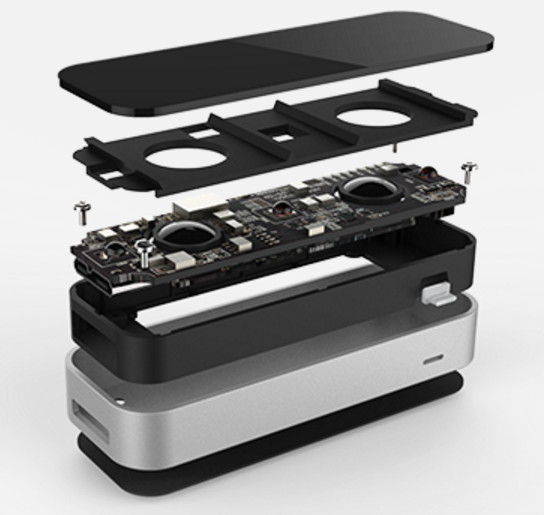
\includegraphics[width=6cm]{Bilder/leap-motion.png}			
		\caption{Aufbau der Leap Motion.~\cite{website:LeapMotionBlog}}
		\label{fig:leapMotion}
\end{figure}


\subsubsection{Würfel Marker}\label{sec:WürfelMarker} \todo[inline, color=green]{Vera}

In vielen VR oder AR Umgebungen müssen die Nutzer eines Systems häufig nach virtuellen Objekten zur Interaktion greifen, die nicht real existieren. Demzufolge greifen die Personen ins Leere, was die Immersion erheblich stört und zu Irritationen sowie Unsicherheit führt.
Um dem Nutzer des Systems \textit{MArC} für die Positionierung und Orientierung ein reales haptisches Feedback zu ermöglichen wurden zwölf Aluminumwürfel mit aufgeklebten Markern entwickelt. Diese Würfel können beliebig innerhalb eines zuvor festgelegten Bereiches auf dem realen Tisch verschoben und rotiert werden. An der aktuellen Position und Orientierung des jeweiligen Markers wird in der VR ein explizit zugeordnetes Objekt gerendert. Diese Position wird mit Hilfe des Tracking-Algorithmus (siehe Kapitel \ref{sec:Tracking}) aus den Bildern der uEye Kamera ermittelt.
Alle zwölf Marker stimmen mit der Form und Farbe, sowie Material und Oberflächenbeschaffenheit aus Abbildung \ref{fig:marker} überein. Sie haben eine Kantenlänge von $46\,mm$ und sind in einem Winkel von $45^\circ$ an allen Kanten gefräst. Das Aluminium ist glasperlgestrahlt um eine matte Oberfläche zu erzeugen, welche ungewollte Reflexionen und Überstrahlungen vermeidet, die unter Umständen den Tracking-Algorithmus beeinflussen können. 

Auf die Oberseite des Markers ist mittig ein leuchtend grünes Quadrat mit einer Kantenlänge von $40\,mm$ aufgebracht. Diese grüne Fläche wird für ein Green-Keying benötigt, welches die Verfolgung der Marker auch bei Bewegungsunschärfe ermöglicht. Die leuchtend grüne Farbe wurde ausgewählt, da sie auf Grund ihrer hohen Leuchtkraft selten in der Natur und vor allem nicht in der Hautfarbe vorkommt. So hebt sie sich stark von ihrer Umgebung ab und erleichtert das Segmentieren der grünen Fläche im Bild. Die rechteckige Form der grünen Flächen hat noch eine weitere Bedeutung. Auf Grund der Geometrie können die äußeren Eckpunkt wie bei den rechteckigen codebasierten Markern auch zur Berechnung der Orientierung des Würfelmarkers im Kameraraum verwendet werden.

Ebenfalls mittig ist jeweils ein individueller $35\,mm$ großer $16$ bit ArUco Marker plan befestigt. Alle verwendeten ArUco-Marker haben einen Rand von einem Bit hat und wurden jeweils aus dem Marker Dictionary $\texttt{DICT\_4X4\_50}$ des ArUco Moduls \cite{website:ArucoDoc} generiert. Die maximale Anzahl an IDs von $50$ ist ausreichend für den Prototypen von \textit{MArC}, da die Anzahl von $50$ Würfelmarkern die durchschnittliche Fläche ausfüllt. Ein weiterer Vorteil dieses verhältnismäßig kleinen Dictonarys ist, dass auch der Aufwand für den entsprechenden Abgleich einer ID mit den potentiellen Mustern im Dictonary erheblich reduziert werden kann. 
Weiterführend beinhaltet das $\texttt{DICT\_4X4\_50}$ Dictionary auf Grund seiner $16$ bit Codierung sehr grobe und einfache Muster, welche gegen die mögliche Bewegungsunschärfe robuster ist. Bei sehr feinen Strukturen kann es schneller zu einer Verwischung des gesamten Musters kommen und die Wahrscheinlichkeit einer erfolgreichen Erkennung sinkt.
	\begin{figure}[H] 
	\center 
	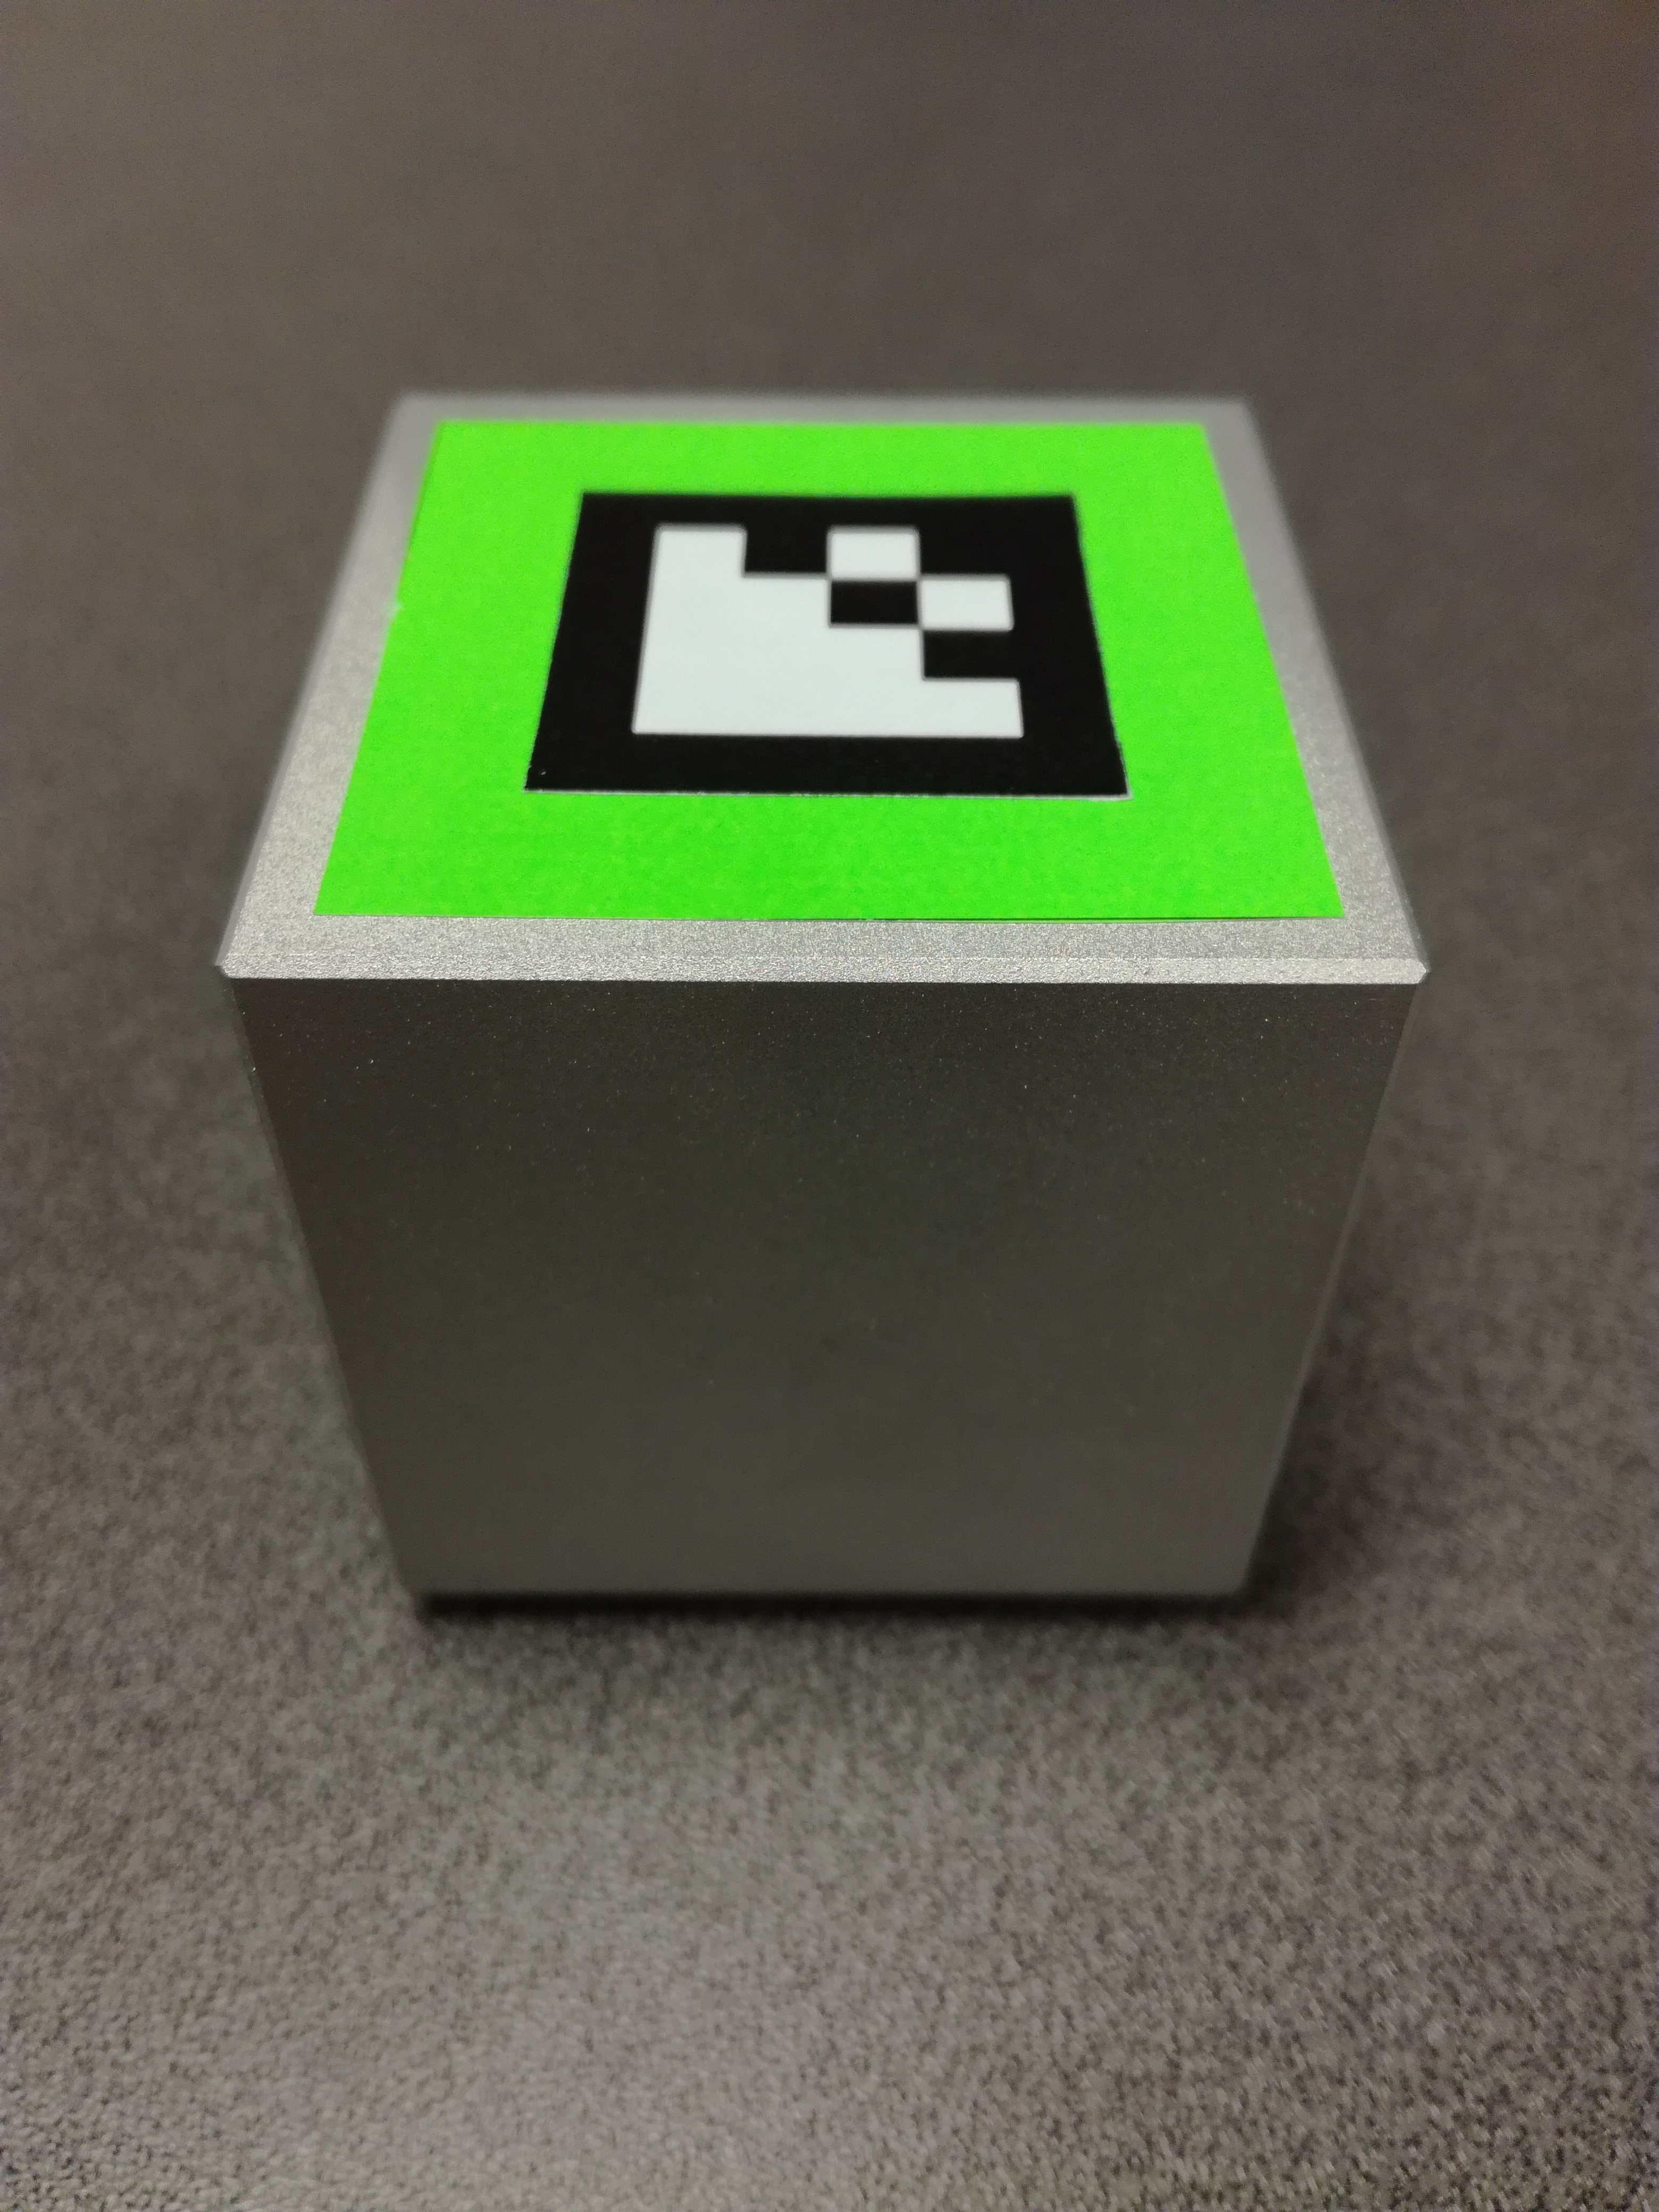
\includegraphics[trim = 0mm 280mm 0mm 150mm, clip, width=6cm]{Bilder/tracking-marker.jpg}			
	\caption{Würfel Marker mit grüner Fläche und einem ArUco Marker, die mittig auf den Aluminumwürfel aufgebracht sind.}
	\label{fig:marker}
\end{figure}

\subsubsection{Schachbrett-Kalibrierungshelfer zur Kamerakalibrierung} \label{sec:SchachbrettKalib} \todo[inline, color=green]{Laura}
Der in Abbildung~\ref{fig:schachbrettKalib} gezeigte Kalibrierungshelfer wird für die Kamerakalibrierung (vgl. Abschnitt~\ref{sec:camCalib}) der \textit{uEye}-Kamera, deren Eigenschaften in Abschnitt~\ref{sec:uEye} beschrieben werden, verwendet. Dazu wurde eine Tisch-artige Erhöhung gebaut, die genauso hoch ist, wie die Würfel-Marker (vgl. Abschnitt~\ref{sec:WürfelMarker}). Darauf ist ein ausgedrucktes Schachbrettmuster mit $8\times10$ Feldern, wobei man algorithmus-bedingt nur die inneren Felder zählt, also $7\times9$ Felder. Dieses steht unter \url{http://www.mrpt.org/downloads/camera-calibration-checker-board_9x7.pdf} (Abgerufen am: 25.03.2017) zum Download bereit.

	\begin{figure}[H] 
	\center 
	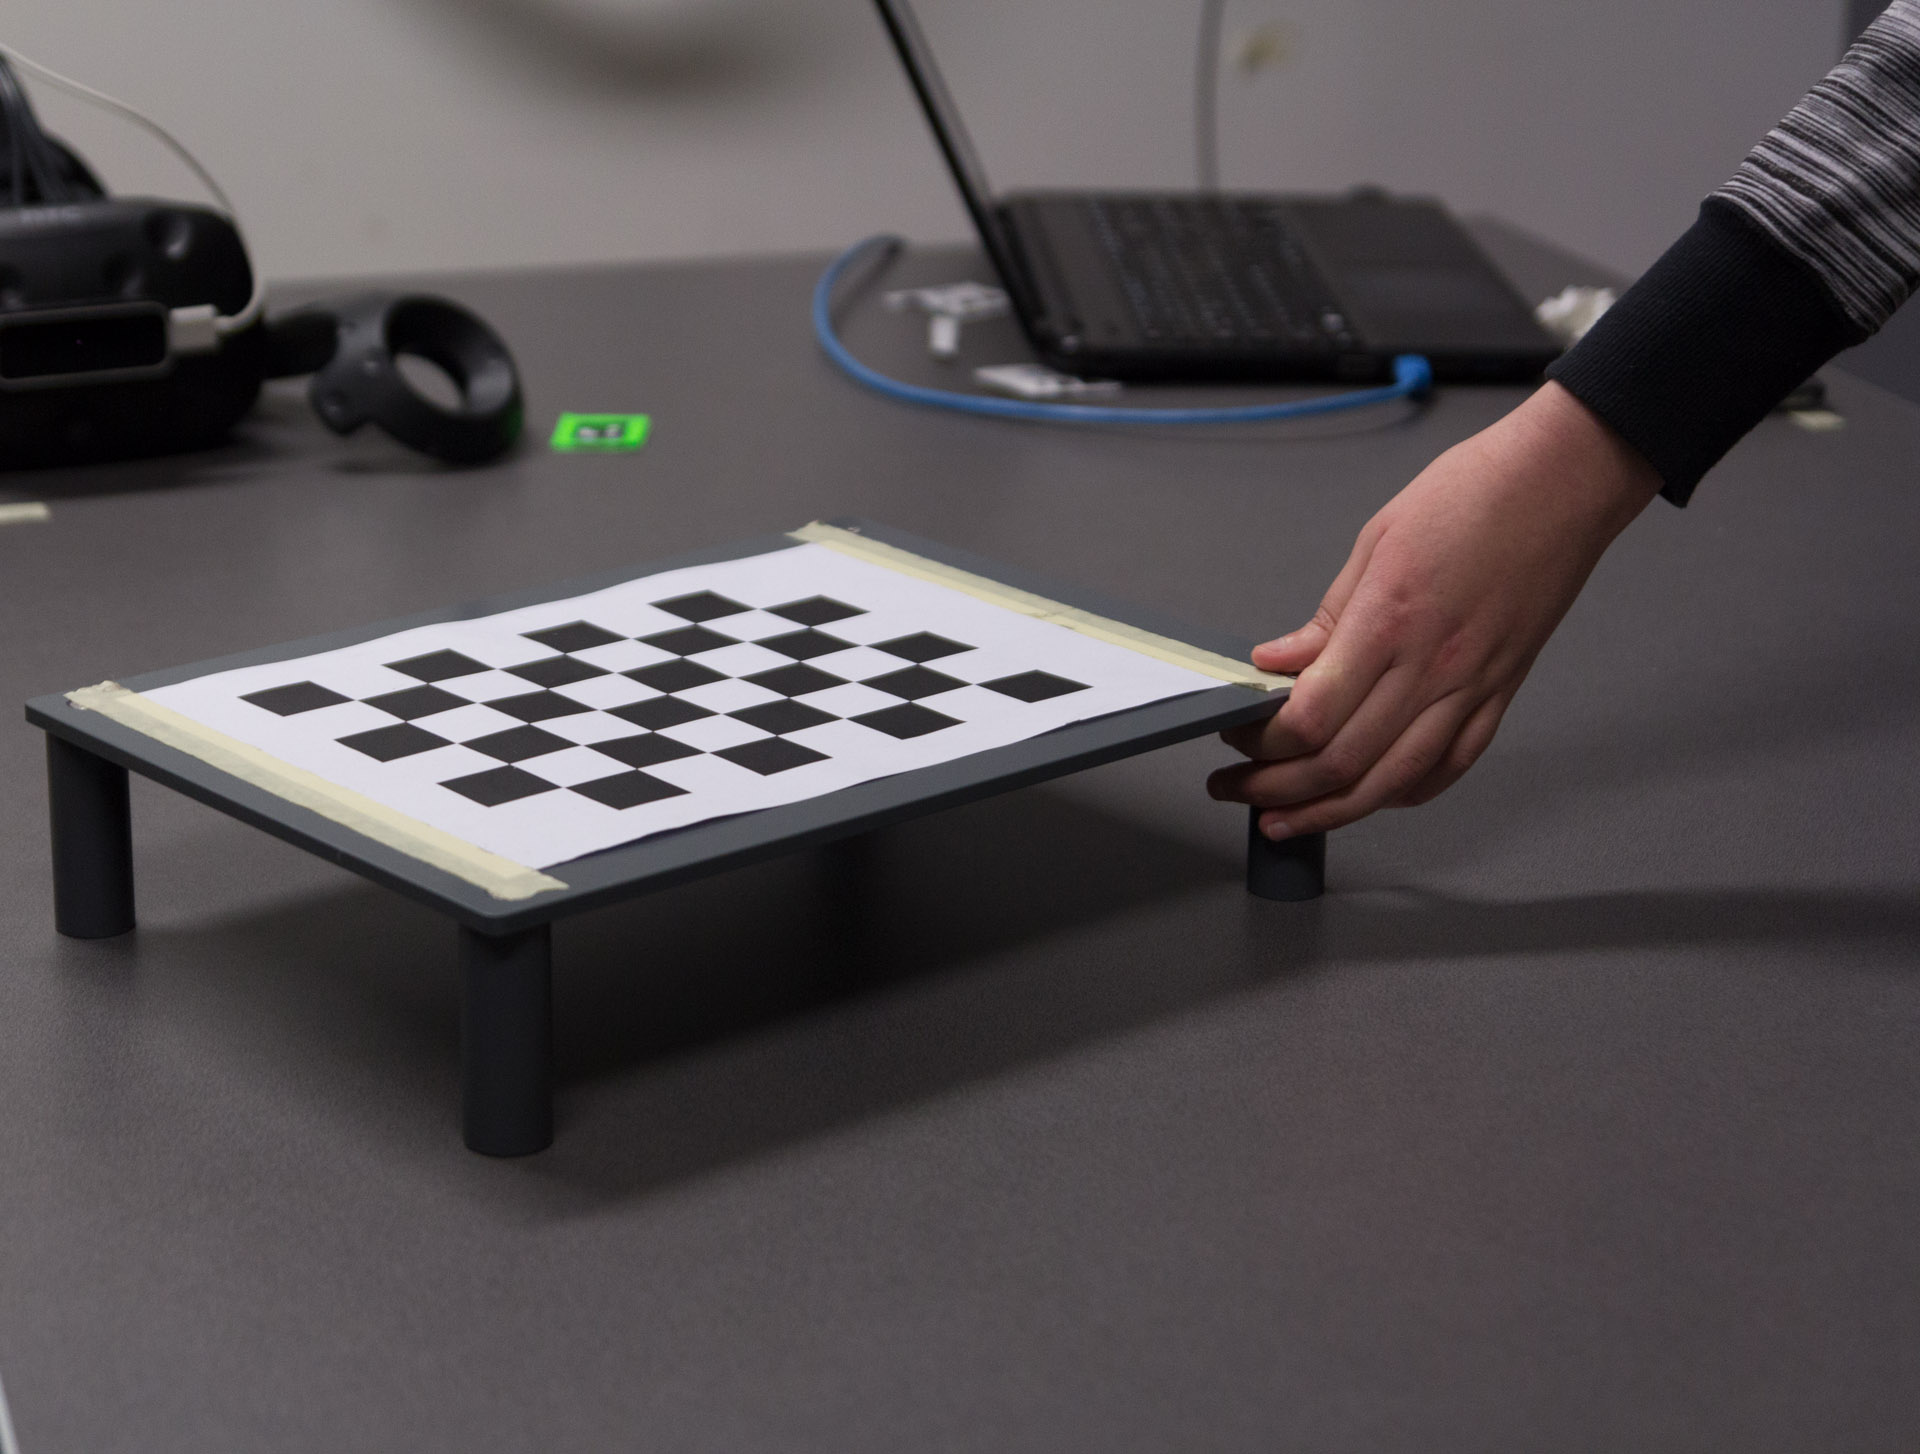
\includegraphics[trim = 0mm 20mm 30mm 40mm, clip]{Bilder/Eigene Fotos/IMG_0004.jpg}			
	\caption{Schachbrett-Kalibrierungshelfer.}
	\label{fig:schachbrettKalib}
\end{figure}

\subsubsection{Kalibrierungscontroller zur Arbeitsbereichskalibrierung} \label{sec:calibController} \todo[inline, color=green]{Laura}
Für die Kalibrierung des Arbeitsbereichs, die in Abschnitt~\ref{sec:planeCalib} beschrieben wird, wurde ein Controller der \textit{HTC Vive} wie in Abbildung \ref{fig:KontrollerMarc} zu sehen verändert. Zum einen wurde ein \textit{ArUco} Marker mit der ID $49$ auf der Oberseite des Controllers befestigt und zum anderen wurde eine Unterlage angefertigt, die verhindern soll, dass der Controller während der Kalibrierung wackelt.\\
Bei der Anbringung des eben erwähnten \textit{ArUco} Markers, der in Abbildung \ref{fig:AllUsedArucoMarker} zu sehen ist, ist die genau Positionierung entscheidend. Er muss genau mittig unter dem Ring des Controllers aufgebracht werden, so wie es auf der Abbildung zu sehen ist. Dies ist entscheidend für die das spätere Verfahren, dass auf korrespondierenden Punktepaaren basiert (vgl. Abschnitt~\ref{sec:Korrespondenz}). Um eine leichtere Aufbringung und gute Ausrichtung des \textit{ArUco} Markers zu vereinfachen, wurde dafür eine kleine Auflagefläche am  Kalibrierungscontroller angebracht. Diese ist so angebracht, dass der Mittelpunkt des \textit{ArUco} Markers sich möglichst genau an der Stelle befindet, wo auch die Position des Controllers aus Unity heraus gemessen wird.

	\begin{figure}[H]
		\centering
		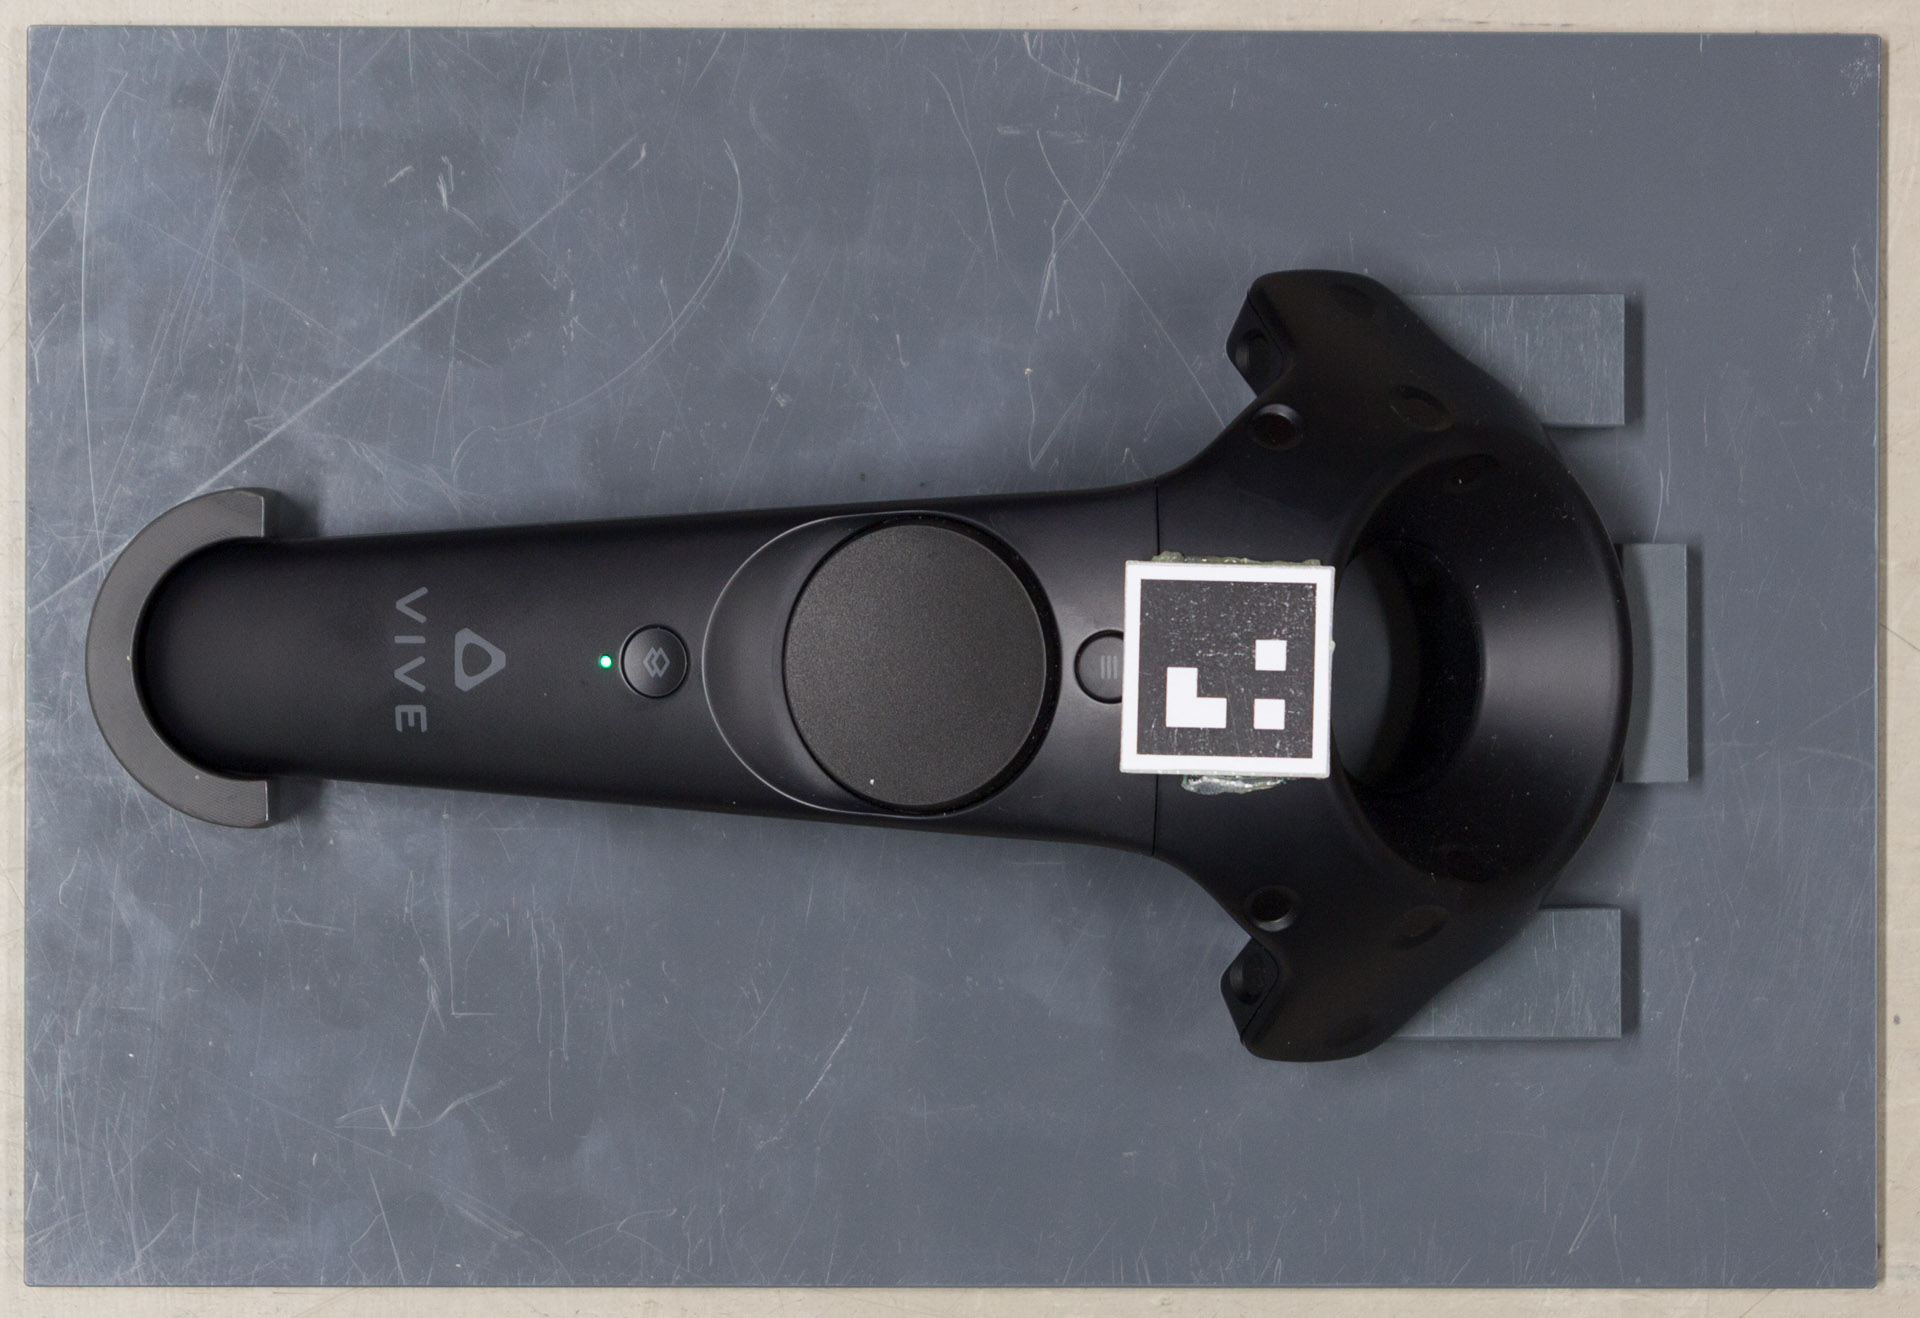
\includegraphics[width=4in]{Bilder/Eigene Fotos/IMG_0032.jpg}
		\caption{Kalibrierungscontroller des \textit{MArC} System mit ArUco Marker.}
		\label{fig:KontrollerMarc}
	\end{figure}
	
\subsection{Obsolete Hardware}\label{sec:obsoleteHardware}\todo[inline, color=green] {Lukas}
Im Laufe eines Projekts nach Art von \emph{MArC} ist es kaum vermeidbar, dass die gesetzten Projektziele reevaluiert werden müssen. Die Gründe hierfür können vielfältig sein. Beispielsweise könnte die Fertigstellung eines bestimmten Teils des Projekts deutlich länger gedauert haben als geplant, oder es könnte sich herausgestellt haben, dass bestimmte Komponenten zueinander nicht kompatibel sind.

Im vorliegenden Projekt trat eine Kombination der beiden oben genannten Gründe auf. Das Betreiben der \emph{Ovrvision Pro} Stereokamera, welche in Abschnitt~\ref{sec:ovrvision} kurz vorgestellt wird, am US-Bus verschiedener während der Entwicklung verwendeter Computer stellte sich als unberechenbar und damit leider unbenutzbar heraus. Die Kamera sorgte während der Ausführung von Unity dafür, dass mit allen anderen Geräten, die ebenfalls per USB angeschlossen waren, unterschiedlichste Probleme auftraten. Als die Situation nach dem Verbinden der Kamera in der teilweisen Zerstörung eines Mainboards gipfelte, wurde die Entscheidung getroffen, die \emph{Ovrvision Pro} nicht länger als Gerät in der Entwicklung von \emph{MArC} zu verwenden.

Stattdessen reifte zu diesem Zeitpunkt die Idee, eine gewöhnliche Webcam zu verwenden, um die Realisierung von Augmented Reality dennoch zu ermöglichen, wenn auch ohne den Stereo-3D-Effekt, welchen die \emph{Ovrvision Pro} nativ bereitgestellt hätte.

Im weiteren Verlauf des Projekts führte eine, lange Zeit ungeklärte, starke Abweichung der Positionen der realen und virtuellen Marker zur Neuordnung der Projektprioritäten. Dies hatte zur Folge, dass letztendlich auch die Webcam als Plattform für die Umsetzung der AR-Fähigkeiten von \emph{MArC} aufgegeben wurde und stattdessen auf eine reine VR-Lösung der Projekt-Problemstellung umgeschwenkt wurde.

Nachfolgend werden die Eigenschaften und technischen Daten beider Geräte kurz beschrieben.
\subsubsection{Ovrvision Pro}\label{sec:ovrvision}\todo[inline, color=green]{Lukas}
Die \emph{Ovrvision Pro} (vgl. Abb.~\ref{fig:ovr}) ist eine kompakte Stereokamera, welche über USB 3.0 mit einem Computer verbunden wird.~\cite{website:ovrvision} Für die Kamera ist eine Vielzahl an Software-Development-Kits (SDKs) für verschiedene Plattformen und Frameworks, wie etwa Microsoft Windows, Linux, Apple Mac OS X, Unreal Engine oder Unity verfügbar.~\cite{website:ovrvisionSetup}

Die \emph{Ovrvision Pro} ist speziell auf Augmented Reality (AR) Anwendungen ausgelegt. So unterstützt die Kamera natives Stereo-3D und bietet auch Bildmodi mit hohen Bildwiederholraten, welche für die Verwendung mit VR-Hardware wie Oculus Rift oder HTC Vive notwendig sind, um die Immersion des Benutzers nicht durch zu träge Bewegungswiedergabe zu beeinflussen. Die unterstützten Bildmodi der Kamera sind in Tabelle~\ref{tab:ovrRes} aufgeführt. Wie aus Abschnitt~\ref{sec:Vive} hervorgeht, stellt die HTC Vive Bildinhalte mit $1080\times1200$\,Pixeln pro Auge bei $90$\,Hz Bildwiederholrate da. Diese Leistung wird von der \emph{Ovrvision Pro} nicht erreicht.

\begin{table}
	\centering
	\begin{tabular}{|c|c|c|c|}
		\hline
		\Absatzbox{}
		\textbf{Örtliche Auflösung}& \textbf{Zeitliche} & \multicolumn{2}{c|}{\textbf{Bildwinkel}}\\
		\cline{3-4}
		\Absatzbox{}
		\textbf{pro Auge}& \textbf{Auflösung} & \textbf{Horizontal} & \textbf{Vertikal}\\
		\hline
		$2560\times1920$\,px & $15$\,fps & $115^\circ$ & $105^\circ$\\
		\hline
		$1920\times1080$\,px & $30$\,fps & $87^\circ$ & $60^\circ$\\
		\hline
		$1280\times960$\,px & $45$\,fps & $115^\circ$ & $105^\circ$\\
		\hline
		$1280\times800$\,px & $60$\,fps & $115^\circ$ & $90^\circ$\\
		\hline
		$960\times950$\,px & $60$\,fps & $100^\circ$ & $98^\circ$\\
		\hline
		$640\times480$\,px & $90$\,fps & $115^\circ$ & $105^\circ$\\
		\hline
		$320\times240$\,px & $120$\,fps & $115^\circ$ & $105^\circ$\\
		\hline
	\end{tabular}
	\caption{Bildmodi der \emph{Ovrvision Pro} Stereokamera.~\cite{website:ovrvisionProduct}}
	\label{tab:ovrRes}
\end{table}


\begin{figure}[H]
	\centering
	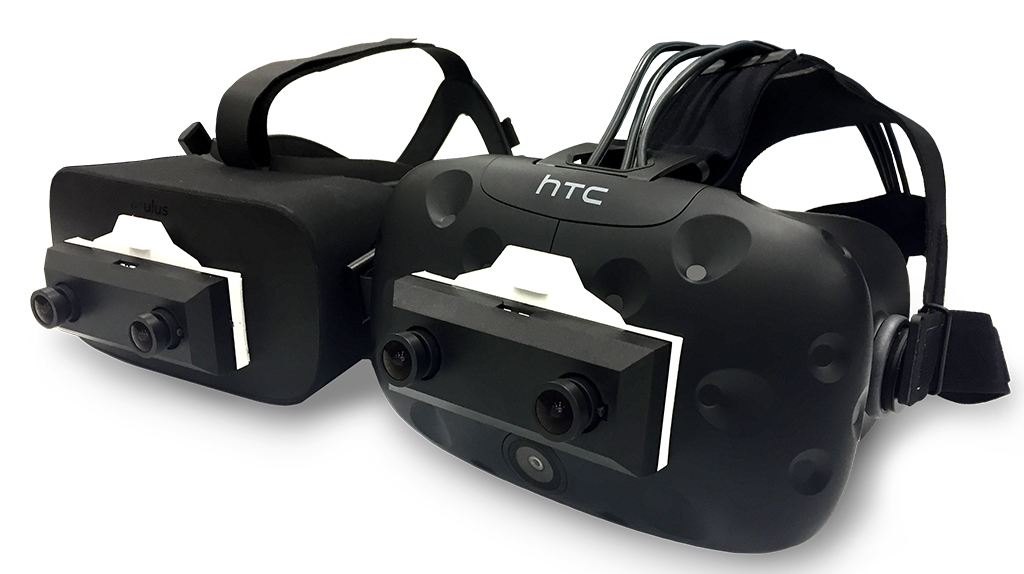
\includegraphics[width=\textwidth]{Bilder/ovr.jpg}			
		\caption{\emph{Ovrvision Pro} Stereokamera montiert an \emph{Oculus Rift} (links) und \emph{HTC Vive} (rechts).~\cite{website:ovrvision}}
		\label{fig:ovr}
\end{figure}
\subsubsection{Webcam}\label{sec:webcam} \todo[inline, color=green]{Vera}

Die \textit{Creative Senz3D} ist eine RGB Kamera mit einer zusätzlichen Infrarot-Tiefenkamera. Das generierte RGB-Bild hat eine Auflösung von $1280\times720$ Pixel und das Tiefenbild von $320\times240$ Pixel bei einer Reichweite von $15\-99\,$cm. Zusätzlich wurde eine Sichtfeld von $74^\circ$ ermittelt. Die Kamera wird über eine USB 2.0 Schnittstelle mit einem Computer verbunden und nimmt Videos mit einer Framerate von bis zu $30$ fps auf \cite{website:Senz3d}. Weiter ist es möglich die Kamera direkt aus Anwendungen per \textit{Intel Perceptual Computing SDK} anzusteuern.

\subsection{Software} \todo[inline, color=green]{Vera}

Zur Entwicklung der \textit{MArC}-Software sind diverse Software-Komponenten und Bibliotheken notwendig. Die Funktionalitäten und Verwendung dieser Komponenten werden in diesem Kapitel kurz erläutert.


\subsubsection{Unity}\label{sec:unity}\todo[inline, color=green]{Lukas}

Unity ist eine sogenannte Spiel-Engine, also eine Entwicklungs- und Laufzeitumgebung, die speziell auf die Entwicklung von 3D-Spielen ausgelegt ist. Die Software wurde am 6. Juni 2005 veröffentlicht \cite{haas2014history} und wird von Unity Technologies \cite{website:Unity} entwickelt und vertrieben. In der Spieleentwicklung ist Unity weit verbreitet, so werden beispielsweise $34\,\%$ der kostenfreien Top-1000-Spiele im mobilen Sektor mit Unity entwickelt \cite{website:UnityPR}.

Unity bietet eine sehr breite Plattformunterstützung \cite{website:UnityMultiPlatform} und erlaubt ebenso die Entwicklung für Head-Mounted-Displays, wie etwa die Oculus Rift \cite{website:UnityOculus}\cite{website:UnityVRoverview} oder auch die in diesem Projekt verwendete HTC Vive \cite{website:UnityVRoverview}.

Die zu Beginn des Projekts verwendete Stereo-Kamera \emph{Ovrvision Pro} stellt ein Software-Development-Kit (SDK) für Unity (Version 5) zur Verfügung \cite{website:ovrvisionSetup}. Da das endgültige Resultat des Projekts die Verwendung der \emph{Ovrvision Pro} nicht mehr vorsieht, wie in~\ref{sec:obsoleteHardware} beschrieben, wird auf eine weitere Beschreibung dieses SDKs verzichtet.

\subsubsection{Visual Studio 2015}\label{sec:VisualStudio} \todo[inline, color=green] {Vera}

\textit{Micosoft Visual Studio 2015} ist eine verbreitete integrierte Entwicklungsumgebung (IDE), welche unter anderem die Programmiersprachen Visual Basic, Visual C$\#$, und Visual C++ unterstützt. Mit Hilfe dieser IDE kann ein Entwickler Win32/ Win64 Anwendungen sowie weitere Web Applikationen und Webservices \cite{website:VisuStud} programmieren und anschließend compilieren. Für \textit{MArC} wurde mit der Version $14.0.25123.00$ Update2 gearbeitet.

\subsubsection{OpenCV} \label{sec:OpenCV} \todo[inline, color=green] {Vera}
\textit{Open Source Computer Vision} (OpenCV) ist eine Open Source Bibliothek für Bild- und Videoverarbeitung in der Programmiersprache \textit{C}$++$. Vorgestellt wurde sie vor über zehn Jahren von \textit{Intel} und wird seitdem stetig von verschiedenen Programmierern weiterentwickelt. Diese Bibliothek stellt die gängigsten Algorithmen sowie aktuelle Entwicklungen der Bildverarbeitung zur Verfügung
\cite{article:OpenCV}.\\
Für dieses System ist vor allem das Modul \texttt{calib3d} \cite{website:Calib3dDoc} und das extra Modul \texttt{aruco} \cite{website:ArucoDoc} verwendet. Das erste Modul \texttt{calib3d}  bietet alle notwendigen Funktionen zur Erstellung, Verwendung und Weiterverarbeitung von intrinsischen und extrinsischen Kamerakalibrierungen an (siehe Kapitel \ref{sec:calib}). Während das Zweite alle benötigten Ressourcen und Funktionalitäten zur Verfolgung von \textit{ArUco} Markern zur Verfügung stellt (siehe Kapitel \ref{sec:aruco}).

%\subsubsection{Orion Beta Software} \label{OBS}\todo[inline] {Paul}
\subsubsection{ArUco Bibliothek} \label{sec:aruco} \todo[inline, color=green]{Vera}
Die ArUco Bibliothek ist ein Marker Tracking Modul von \textit{OpenCV} (siehe Kapitel \ref{sec:OpenCV}) kann für Augmented Reality (AR) Anwendungen genutzt werden und stellt für diese Anwendungen alle notwendigen Funktionalitäten zum Orten und Verifizieren der Codes sowie einer Positionsabschätzung der ermittelten Positionen im Kameraraum zur Verfügung \cite{article:Aruco2014}. 
Die Marker bestehen ähnlich wie QR-Codes aus einer zweidimensionalen Matrix, mit schwarzen oder weißen Feldern, welche die kodierten Daten binär, wie in Abbildung \ref{fig:AllUsedArucoMarker}, darstellen.  Weiterführend kann die Bitanzahl (siehe Abbildung \ref{fig:SizesArucoMarker}) und die gefragte maximale Markeranzahl variabel gewählt werden. An dieser Stelle ist eine kleine  Bitanzahl, welche detailarme Muster erzeugt, für eine gute Erkennbarkeit in sehr großen Entfernungen zur Kamera oder kleinen Bildern sinnvoll. Um diese Vielzahl an verschiedenen Größen und IDs zu verwalten wurden sogenannte Dictionarys eingeführt \cite{article:ArucoDictGarridoJurado2015}. Diese Dictionarys bestehen aus Markern mit gleicher Bitanzahl und sind zusätzlich auf eine maximalen Anzahl von IDs begrenzt um ein möglichst hohe Performanz während des Zuordnungsprozesses zu gewährleisten.\\

\begin{figure}[H] 
	\center 
	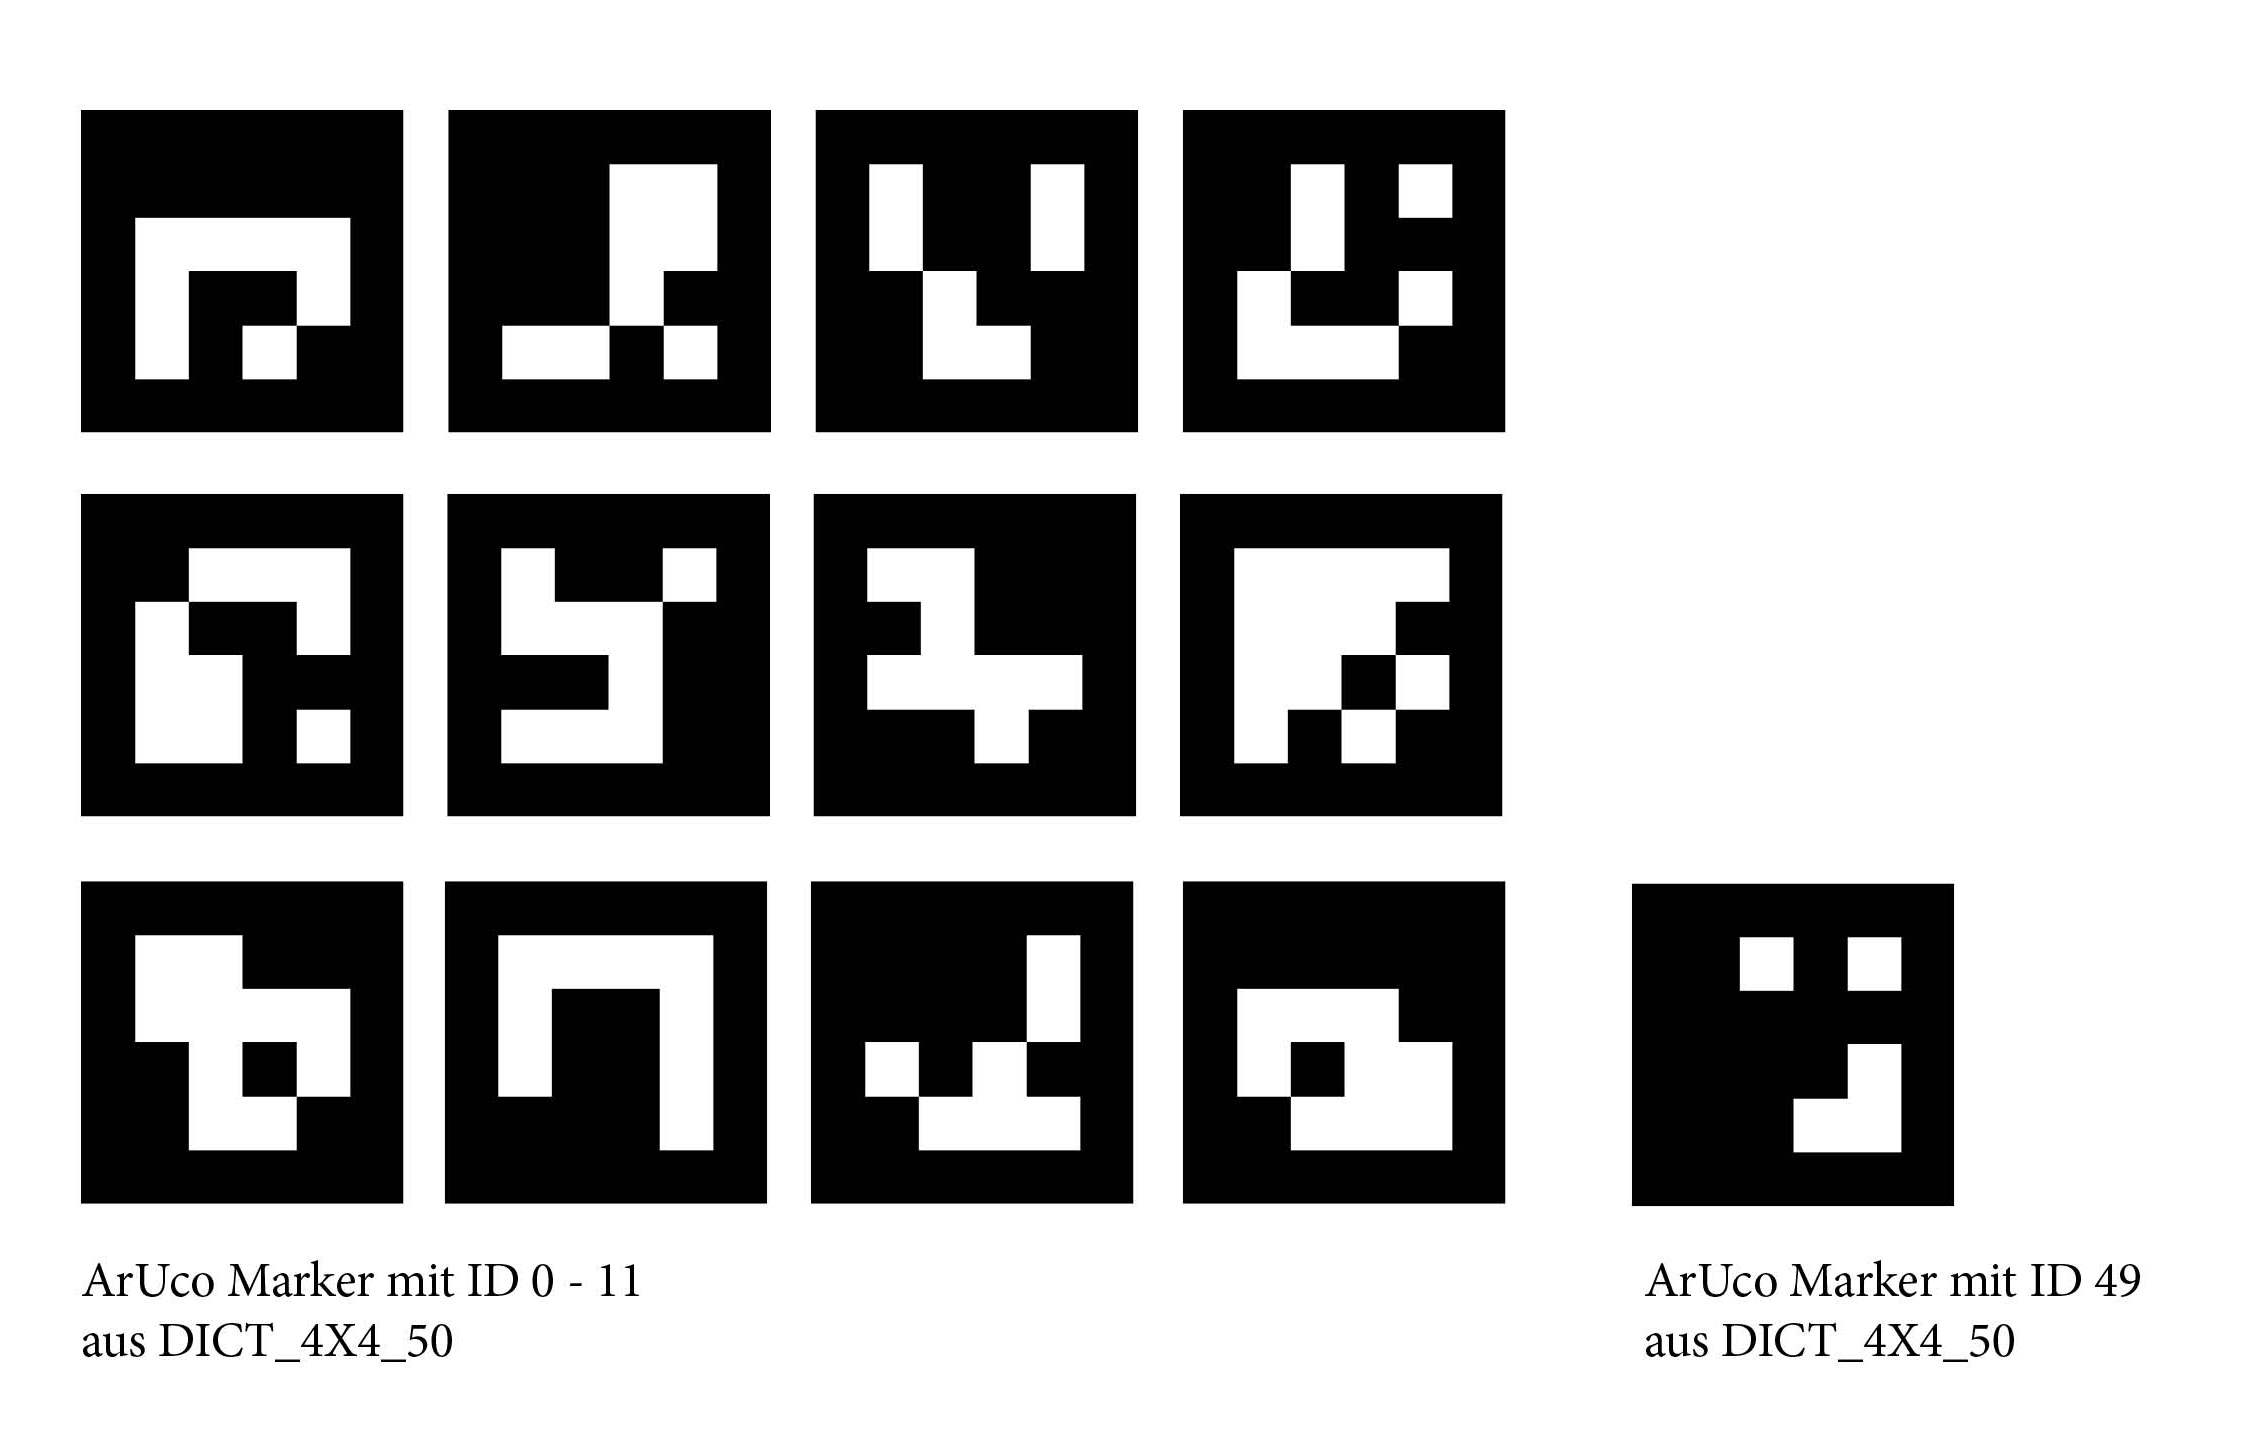
\includegraphics[width=10cm]{Bilder/Aruco_marker.jpg}			
	\caption{Alle genutzten 16 bit ArUco Marker des Prototypen. Links die zwölf IDs der Würfel Marker und rechts die ID, welche zur Kalibrierung benötigt wird. Die maximale Anzahl der Marker ist auf $50$ begrenzt.}
	\label{fig:AllUsedArucoMarker}
\end{figure}

\begin{figure}[H] 
	\center 
	
\includegraphics[width=7cm]{Bilder/VerschAruco.jpg}			
	\caption{ArUco Marker mit unterschiedlicher Bitgröße. Von Links nach Rechts: $n=5$, $n=6$ und $n=8$. Quelle: \cite{article:Aruco2014}}
	\label{fig:SizesArucoMarker}
\end{figure}

\subsubsection{Steam VR}\todo[inline,color=green] {Paul}
\textit{Steam VR} ist die Schnittstelle zwischen der \textit{HTC Vive} und \textit{Unity}. Um das HMD nutzen zu können, musss \textit{Steam VR} auf dem Computer installiert sein. Für den Nutzer ist ein kleines GUI Element auf dem Monitor sichtbar, welches den Status der Geräte der \textit{Vive} darstellt. Hierdurch werden Fehlermedlungen kommuniziert, Kalibrierungen durchgeführt eine Kommunikation mit dem HMD bereitgestellt, so dass das Gerät im Fall der Fälle neugestartet werden kann.\\
Innerhalb von \textit{Unit} stellt \textit{Steam} ein Plugin zur Verfügung, welches direkt in Szenen in \textit{Unity} eingebettet werden kann. Der Entwickler ist also in der Lage, eine vorhandene \textit{Unity}-Szene um die VR Mölglichkeit bequem per Drag and Drop zu erweitern.\\
Das bereitgestellte \textit|{Unity} Prefab beinhaltet alle notwendigen Elemente um mit der Hardware kommunizieren zu können. Dabei wird eine Positionsbestimmung ebenso wie ein Kamerarig für die stereoskopische Bildwiedergabe bereitgestellt, wie auch die Controllereingabe und weiterverwendung der Datenj möglich gemacht.


\subsubsection{Windows Sockets (Winsock)}\label{sec:Winsock}\todo[inline, color=green] {Lukas}
Windows Sockets (abgekürzt Winsock) ist eine API für den Zugriff auf Netzwerkkomponenten in Microsoft Windows Betriebssystemen~\cite{quinn1998windows}. Winsock wird nativ in Microsoft Windows bereitgestellt.\\ 
Für die unkomplizierte Übertragung zwischen zwei Anwendungen in einem lokalen Netzwerk bieten sich sowohl das \emph{Transmission Control Protocol} (TCP), als auch das User \emph{User Datagram Protocol} (UDP) an. Das Erstellen von Netzwerk-Sockets für die Übertragung per TCP und UDP wird von Winsock ermöglicht.\\ Die Umsetzung der Netzwerkverbindung in \emph{MArC} wird in Abschnitt~\ref{sec:netzwerk} näher beschrieben.


\subsubsection{Leap Motion SDK} \label{sec:LeapSDK}\todo[inline, color=green] {Paul}
\textit{Leap Motion Inc.} bietet ein vollständiges Software Development Kit (SDK) für die \textit{Leap} an, welches \textit{Unity} um das Hand- und Fingertracking erweitert. Die Treibersoftware interpretiert die von den Kameras gelieferten Daten und sendet Trackinginformationen an die jeweilige Software. Das Leap SDK setzt an dieser Stelle an und verwendet diese eingehenden Daten um sie auf ein Handmodell in \textit{Unity} zu übertragen. Das SDK ist so vorbereitet, dass der Nutzer fertige Bausteine in die virtuelle Szene einbinden kann, die sich dann um die Dateninterpretation und visualisierung als Handmodelle kümmert. Die Handmodelle, die das SDK liefert, sind mit Collidern ausgestattet. Diese abstrahierte Geometrie lässt \textit{Unity} Kollisionen feststellen. Dieses Feature wird bei \textit{MArC} verwendet, um die Interaktion mit den virtuellen Menüelementen zu realisieren.\\
\textit{Leap} bietet zudem mehrere sog. "Module" an, die das SDK erweitern können. Unter anderem auch ein Modul, welches die \textit{Unity}-internen GUI Elemente mit den Handmodellen bedienbar machen. Nach einigen Tests hat sich jedoch herausgestellt, dass diese Interaktionsmöglichkeit für \textit{MArC} ungeeignet ist, da sie zu instabil läuft. Das um das UI Modul erweiterte SDK projiziert die Position der Fingerspitzen auf die UI Ebene, falls sich die Hand in der Nähe dieser befindet. Auf der UI wird dann ein kleiner Kreis angezeigt, um dem Nutzer ein visuelles Feedback zu gewährleisten.\\
Im Falle von \textit{MArC} sollten die virtuellen UI Elemente auf den Tisch platziert werden. Hierbei sind die Elemente jedoch immer ein wenig oberhalb des Tisches platziert, damit sie in jedem Fall mit der virtuellen Hand bedient werden können. Zwingend durchdringt die Hand dann die UI Elemente. Mittels des mitgelieferten UI-Modules ist eine Interaktion dann nicht mehr möglich. Daher war eine Bedienung mit Hilfe der Collider sinnvoller.

\newpage
\section{System}\todo[inline, color=green]{Lukas}
Die Benutzung von \textit{MArC} ist in der dem Programm mitgelieferten ReadMe-Datei (vgl.~\ref{sec:readMe}) beschrieben. Darin wird erklärt, welche Hard- und Softwarekomponenten erforderlich sind und wie das System gestartet und kalibriert wird. Auf diese Aspekte wird in den folgenden Abschnitten näher eingegangen.\\ 
Des weiteren enthält die ReadMe-Datei eine Übersicht über die enthaltenen Quellcode-Dateien.
\subsection{Aufbau}\label{sec:Aufbau}\todo[inline, color=yellow]{Lukas und Vera}
Der Aufbau von \textit{MArC} kann in zwei Teile aufgeteilt werden. Zum Einen den Part der für das Tracking der Würfel Marker verantwortlich ist und zum Anderen den zweiten Teil, welcher die VR Umgebung erzeugt und die notwendige Peripherie für die Interaktionen stellt.\\
\subsubsection{Tracking Aufbau}\todo[inline, color=green]{Vera}
Wie in Abbildung \ref{fig:AufbauMarc} dargestellt ist wird senkrecht über einem beliebigen Tisch eine Kamera installiert, die Würfel Marker aus der Vogelperspektive filmt. Der Abstand zum Tisch sollte so gewählt werden, dass die Aufnahmen noch scharf sind und sich die Nutzer nicht den Kopf daran stoßen können. Hier ist besondere Vorsicht geboten, da die Nutzer durch die \textit{HTC Vive} nicht die reale Umgebung wahrnehmen können. Für den Prototypen wurde eine \textit{IDS uEye 164LE-C} (siehe Kapitel \ref{sec:uEye}) verwendet und über eine USB 2.0 Schnittstelle an den Computer mit dem Tracking Algorithmus verbunden. Diese Kamera wird mit Hilfe der uEye-API vom Tracking Algorithmus im Live-Bild-Modus initialisiert und gesteuert. In diesen Live Bildern werden die Würfel Marker erkannt und verfolgt. Für jeden erkannten Würfel Marker werden alle relevanten Informationen über die TCP Netzwerkverbindung (siehe Kapitel \ref{sec:Netzwerk}) an den Computer zur Ausführung der \textit{Unity}-Simulation (siehe Kapitel \ref{sec:UnityComp}) übertragen. Damit der Algorithmus einen Würfel Marker erkennt muss er in dem vorab definierten Spielfeld bewegt werden. Diese Festlegung findet während der Kalibrierung des Arbeitsbereiches statt. Für diese Kalibrierung ist es notwendig den einzelnen \textit{ArUco} Marker aus Abbildung \ref{fig:AllUsedArucoMarker} mit der ID $49$ exakt wie in Abbildung \ref{fig:KontrollerMarc} auf den Controller der \textit{HTC Vice} zu montieren, da nur so gewährleistet werden kann, dass die erkannte \textit{ArUco} Marker Position in der Kamerawelt mit den Controller Positionen in der \textit{Unity} Welt korrespondieren.

\begin{figure}[H]
	\centering
	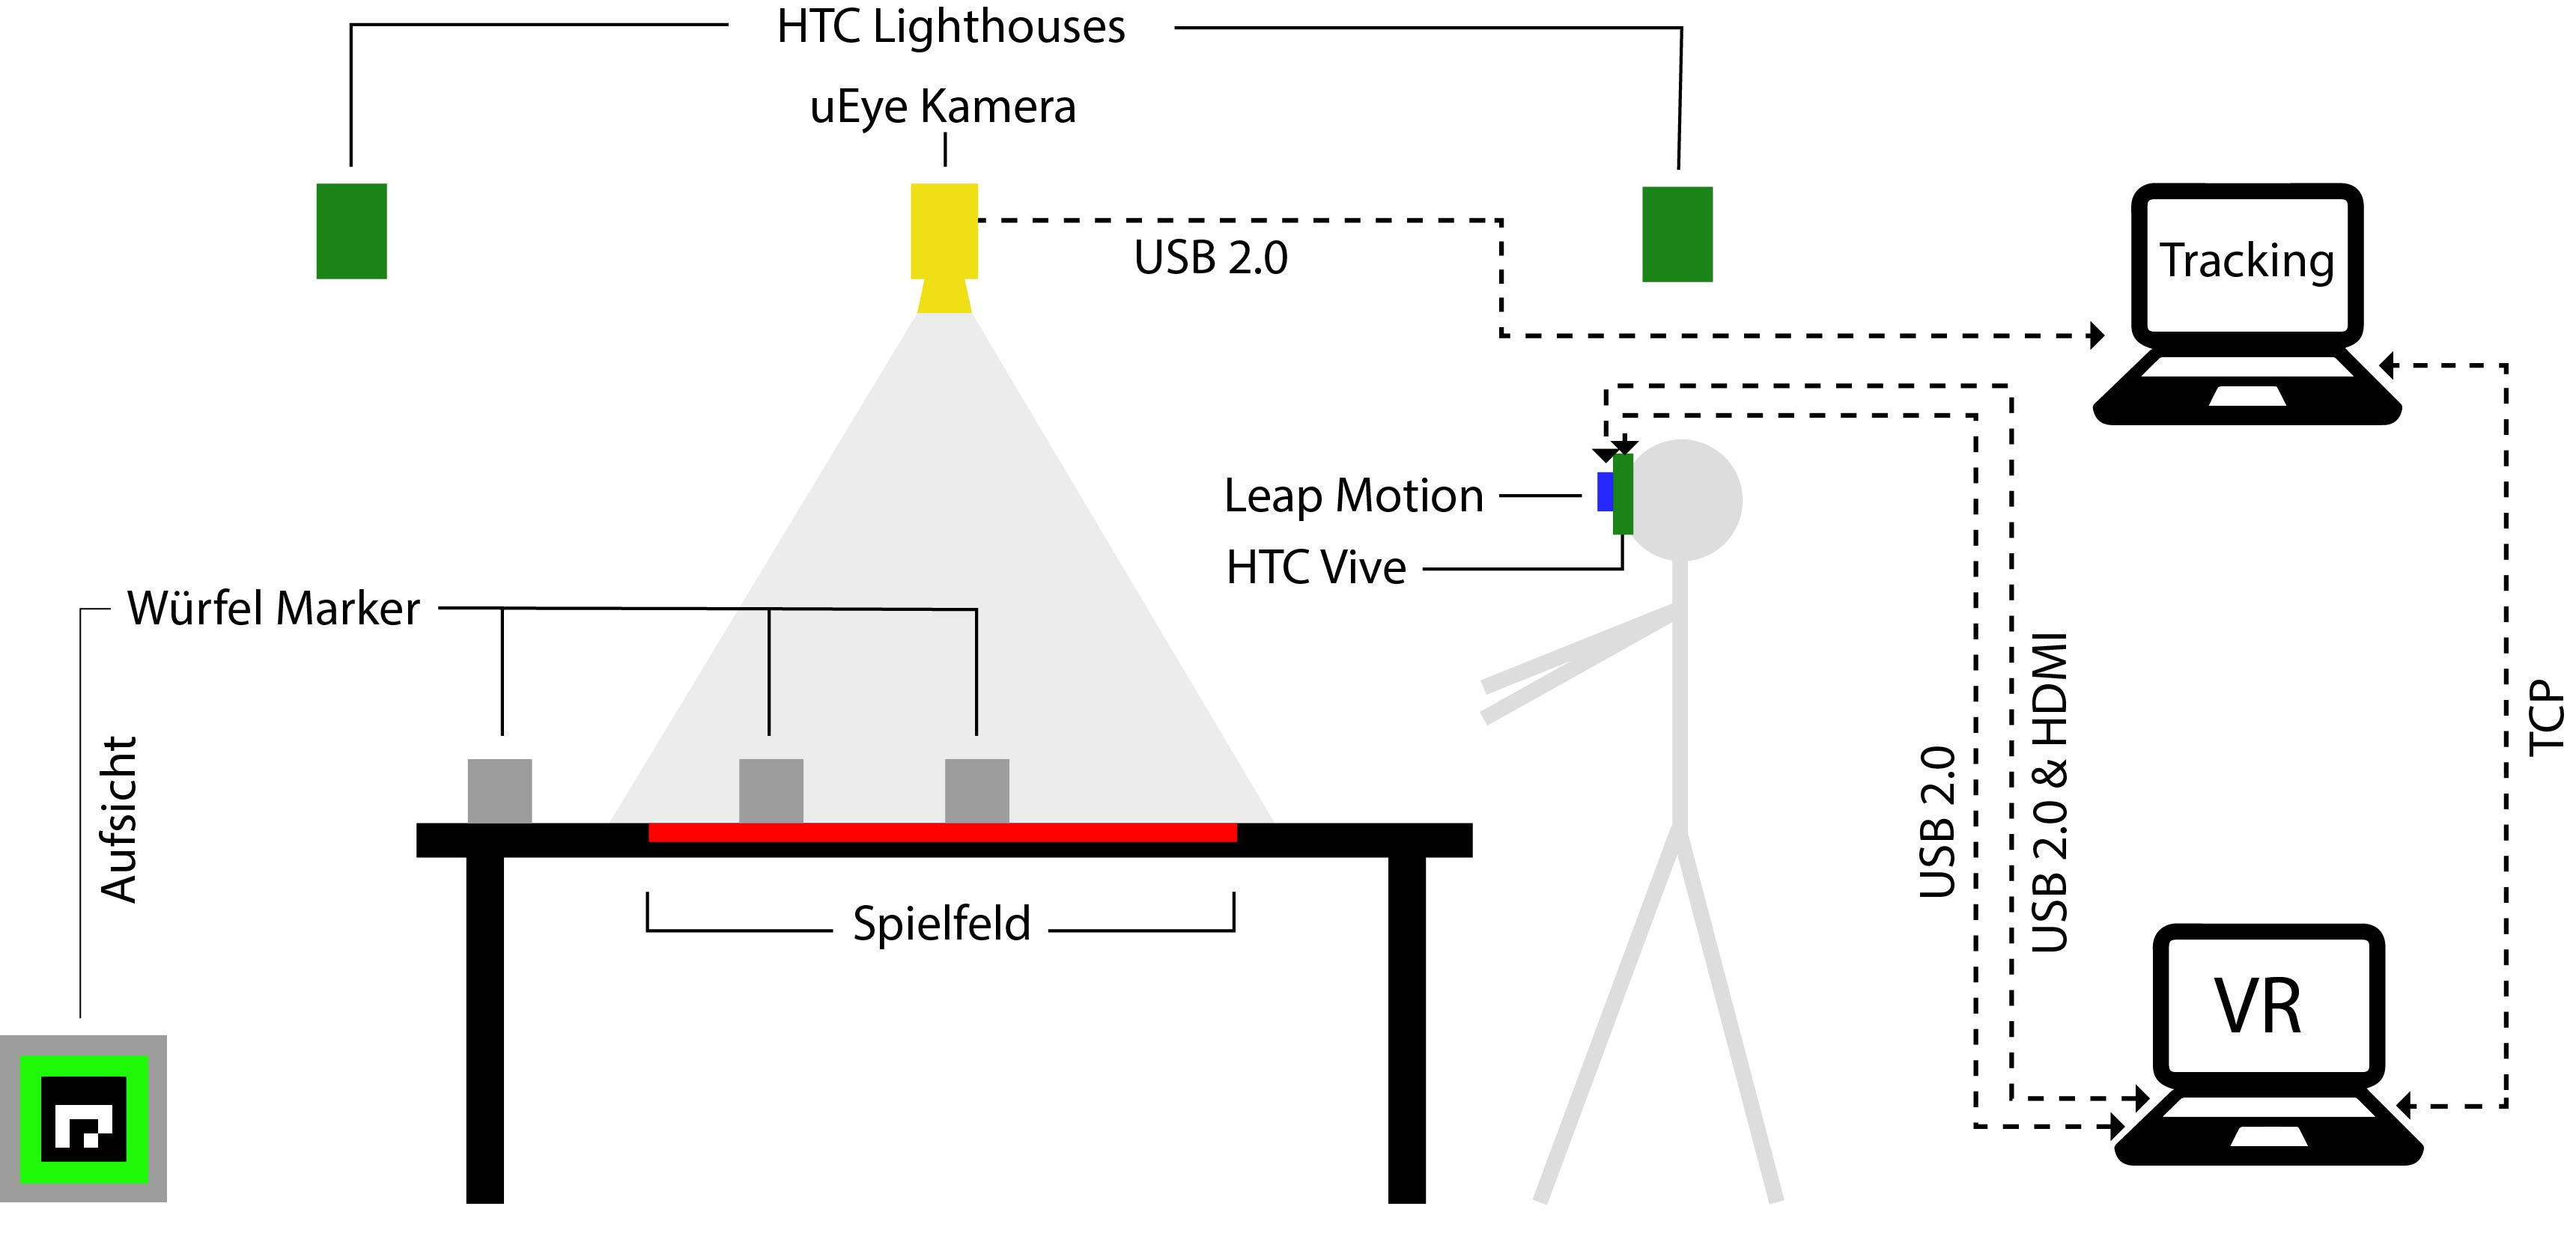
\includegraphics[width=\textwidth]{Bilder/Aufbau_MArC.jpg}
	\caption{Aufbau des \textit{MArC} System.}
	\label{fig:AufbauMarc}
\end{figure}

\begin{figure}[H]
	\centering
	
\includegraphics[width=4in]{Bilder/CalibController.jpg}
	\caption{Kalibrierungscontroller des \textit{MArC} System mit ArUco Marker.}
	\label{fig:KontrollerMarc}
\end{figure}

\subsection{Systemvoraussetzungen}\label{sec:sysVor}\todo[inline, color=green]{Lukas}
Die Systemvoraussetzungen für \emph{MArC} sind in der ReadMe-Datei beschrieben, welche der im Projekt erstellten Software mitgeliefert ist. Die gesamte ReadMe-Datei ist in Abschnitt~\ref{sec:readMe} zu finden, außerdem enthält Abbildung~\ref{fig:marcReadMe} einen Ausschnitt der ReadMe-Datei, welcher die Voraussetzungen beschreibt, die vor dem Starten des Systems erfüllt sein müssen.

\begin{figure}
	\centering
	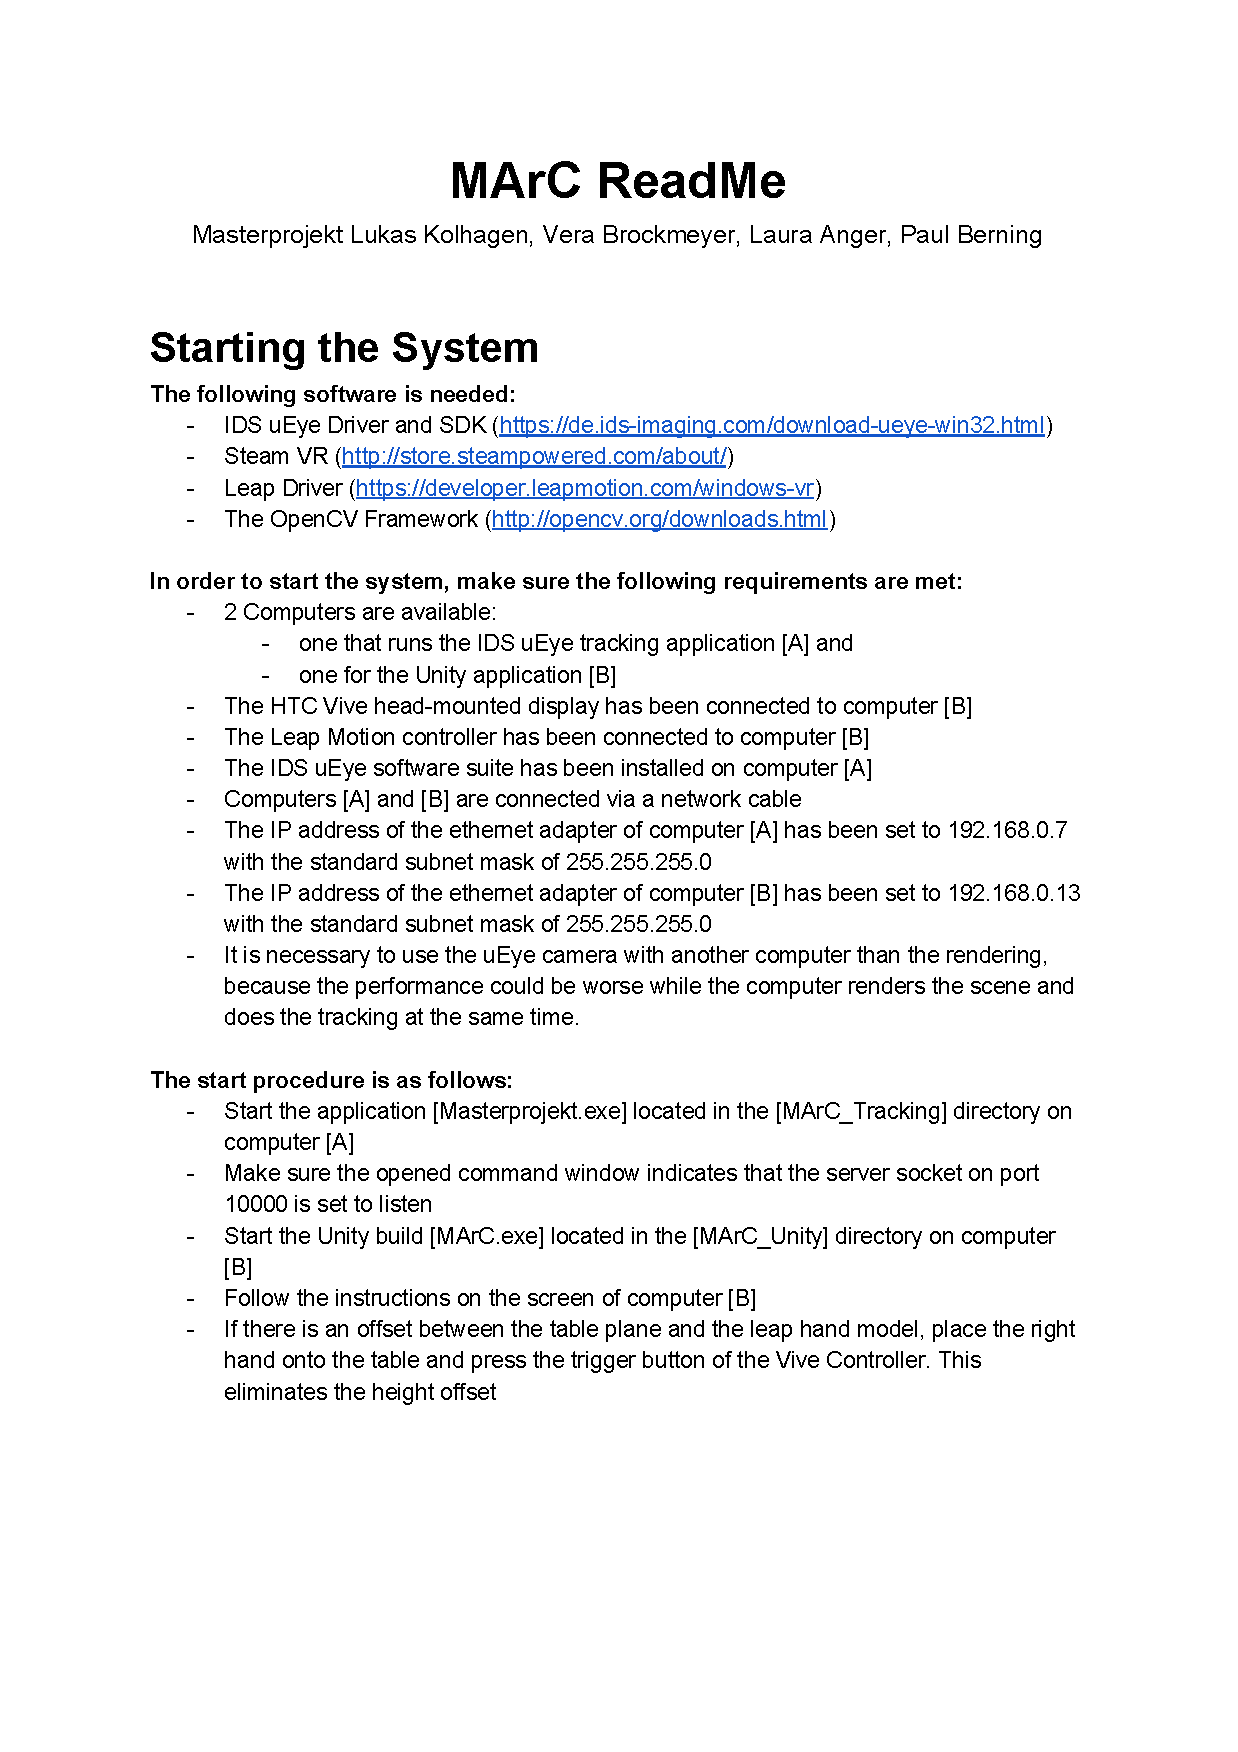
\includegraphics[page=1, trim=1cm 12.25cm 1cm 5.25cm, clip, width=\textwidth]{kapitel/anhang/ReadMe.pdf} 
	\caption{Auszug aus der \emph{MArC} ReadMe-Datei (vgl.~\ref{sec:readMe}).}
	\label{fig:marcReadMe}
\end{figure}

\subsection{Netzwerk}\todo[inline, color=yellow]{Lukas und Laura}

Die in Kapitel \ref{sec:Winsock} beschriebene API verfügt, wie dort geschildert, über die Möglichkeit den Datentransport mittels TCP oder UDP umzusetzen. Für \emph{MaRC} wurde ein TCP-Socket-Netzwerk bestehend aus einem Server und einem Klienten verwendet, weil der der in~\ref{sec:Netzwerk} beschriebene Fehlerschutz des TCPs ausgenutzt werden sollte. Da die zu übertragenden Daten von \emph{MArC} in der Größe exakt definiert und hinreichend klein sind, wurde die etwas höhere Geschwindigkeit einer UDP-Socket-Verbindung als unnötig erachtet.

\todo[inline, color=yellow]{Kann noch angepasst wereden und muss noch erweitert werden}

\subsection{Starten des Systems}\todo[inline, color=green]{Lukas}
Nachdem sichergestellt wurde, dass alle in~\ref{sec:sysVor} beschriebenen Voraussetzungen bestehen, kann das System gestartet werden, indem zunächst die Tracking-Anwendung (auf dem einen Computer, vgl.~\ref{sec:TrackingComp}) und anschließend die aus Unity heraus erstellte Anwendung (auf dem anderen Computer, vgl.~\ref{sec:UnityComp}) gestartet wird. Auf letzterem Computer beginnt darauffolgend die Menüführung, welche in \ref{sec:menu} beschrieben ist. 
\subsection{Menüführung}\label{sec:menu}\todo[inline, color=green]{Lukas}
Die Menüführung dient dazu, den Benutzer durch alle notwendigen Schritte zu leiten, die vor dem Starten der eigentlichen Simulation erforderlich sind. Im nachfolgenden Abschnitt~\ref{sec:menus} werden alle verfügbaren Menüs der Anwendung aufgelistet und kurz beschrieben, während im Abschnitt~\ref{sec:menuAblauf} der Ablauf der Menüführung erläutert wird.


\subsubsection{Menüs}\label{sec:menus}\todo[inline, backgroundcolor=green]{Laura}
Die folgenden Menüs sind Bestandteil der Menüführung:

\begin{minipage}{0.6\textwidth}
	\begin{figure}[H] 
		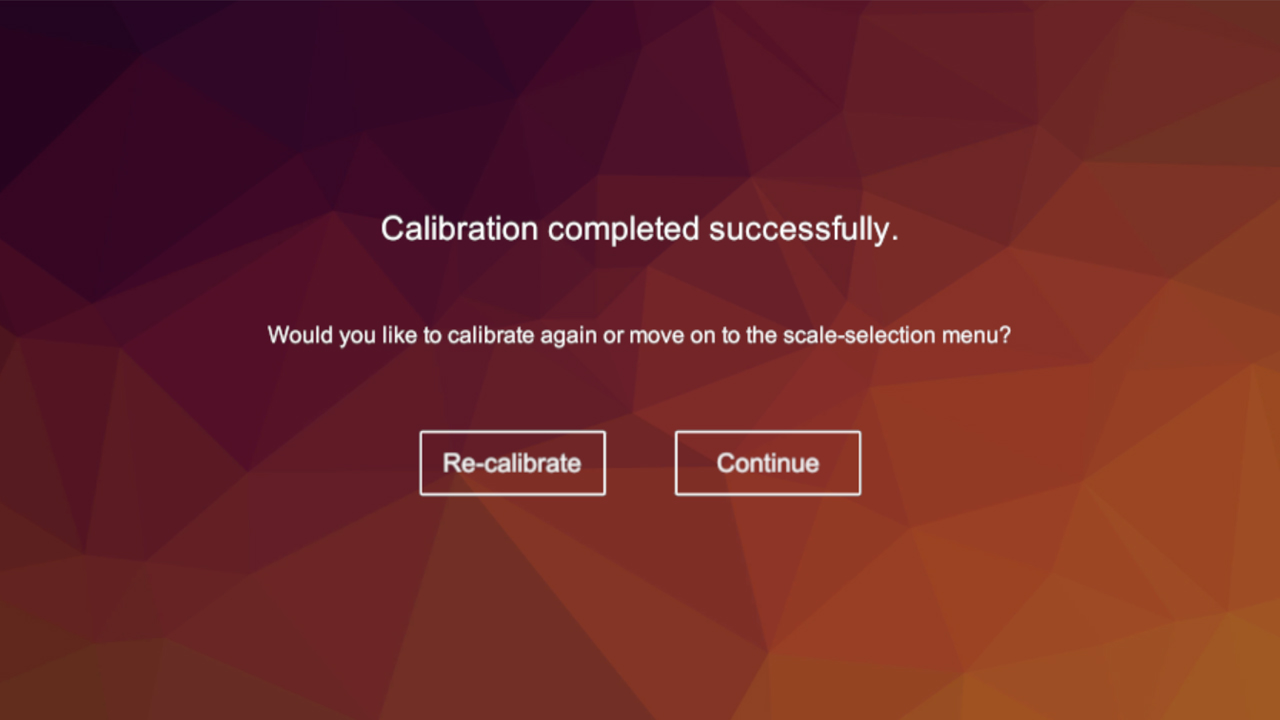
\includegraphics[trim=3cm 2cm 3cm 2cm, clip, width=0.9\textwidth]{Bilder/CalibDone.jpg}
			\label{fig:CalibDone}
	\end{figure}
\end{minipage}
\begin{minipage}{0.4\textwidth}
	\texttt{CalibDone}:\\
	Wird aufgerufen, wenn die Kalibrierung des Arbeitsbereichs abgeschlossen ist. Es informiert den Benutzer, dass die Kalibrierung erfolgreich war und der Vorgang fortgesetzt werden kann.
\end{minipage}\\

\begin{minipage}{0.6\textwidth}
	\begin{figure}[H] 
		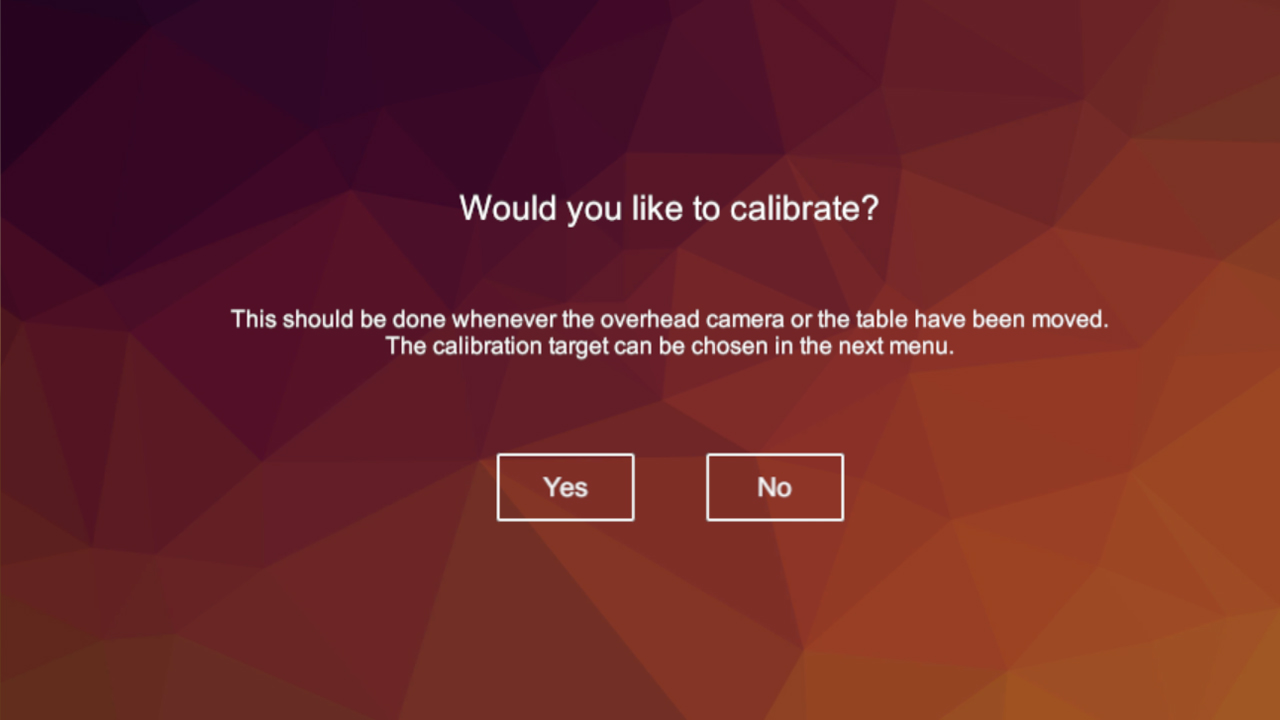
\includegraphics[trim=3cm 2cm 2cm 2cm, clip, width=0.9\textwidth]{Bilder/CalibrateOrNot.jpg}
			\label{fig:CalibrateOrNot}
	\end{figure}
\end{minipage}
\begin{minipage}{0.4\textwidth}
	\texttt{CalibrateOrNot}:\\
	Erscheint nach dem Verlassen des \texttt{Welcome}-Menüs und erlaubt dem Benutzer eine Kalibrierung durchzuführen oder eine bereits durchgeführte Kalibrierung zu laden.
\end{minipage}\\

\begin{minipage}{0.6\textwidth}
	\begin{figure}[H] 
		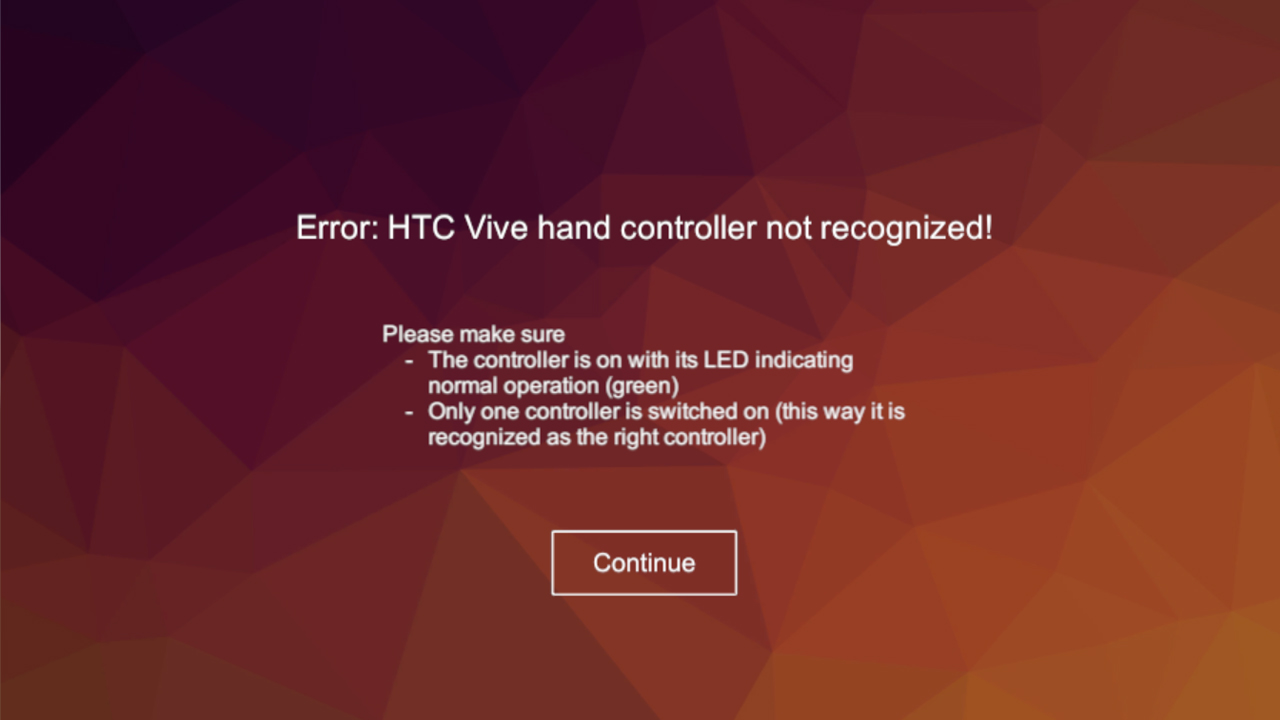
\includegraphics[trim=3cm 1cm 3cm 3cm, clip, width=0.9\textwidth]{Bilder/ControllerNotFound.jpg}
			\label{fig:ControllerNotFound}
	\end{figure}
\end{minipage}
\begin{minipage}{0.4\textwidth}
	\texttt{ControllerNotFound}:\\
	Warnt den Benutzer nach dem Starten der Kalibrierung, dass der HTC Vive Controller, welcher für die Kalibrierung benötigt wird, nicht eingeschaltet ist. Während das Menü angezeigt wird, kann der Benutzer den Controller einschalten und anschließend auf \texttt{Continue} klicken.
\end{minipage}\\

\begin{minipage}{0.6\textwidth}
	\begin{figure}[H] 
		\includegraphics[trim=3cm 1cm 3cm 3cm, clip, width=0.9\textwidth]{Bilder/doPlaneCalibInVS.jpg}
			\label{fig:doPlaneCalibInVS}
	\end{figure}
\end{minipage}
\begin{minipage}{0.4\textwidth}
	\texttt{doPlaneCalibInVS}:\\
	Dient dem Benutzer als Anleitung für die Durchführung der Arbeitsbereich-Kalibrierung. Diese wird in \ref{sec:planeCalib} genauer beschrieben.
\end{minipage}\\

\begin{minipage}{0.6\textwidth}
	\begin{figure}[H] 
		\includegraphics[trim=3cm 2cm 3cm 2cm, clip, width=0.9\textwidth]{Bilder/doPoseCalibInVS.jpg}
			\label{fig:doPoseCalibInVS}
	\end{figure}
\end{minipage}
\begin{minipage}{0.4\textwidth}
	\texttt{doPoseCalibInVS}:\\
	Dient dem Benutzer als Anleitung für die Durchführung der Kamera-Kalibrierung. Diese wird in \ref{sec:camCalib} genauer beschrieben.
\end{minipage}\\

\begin{minipage}{0.6\textwidth}
	\begin{figure}[H] 
		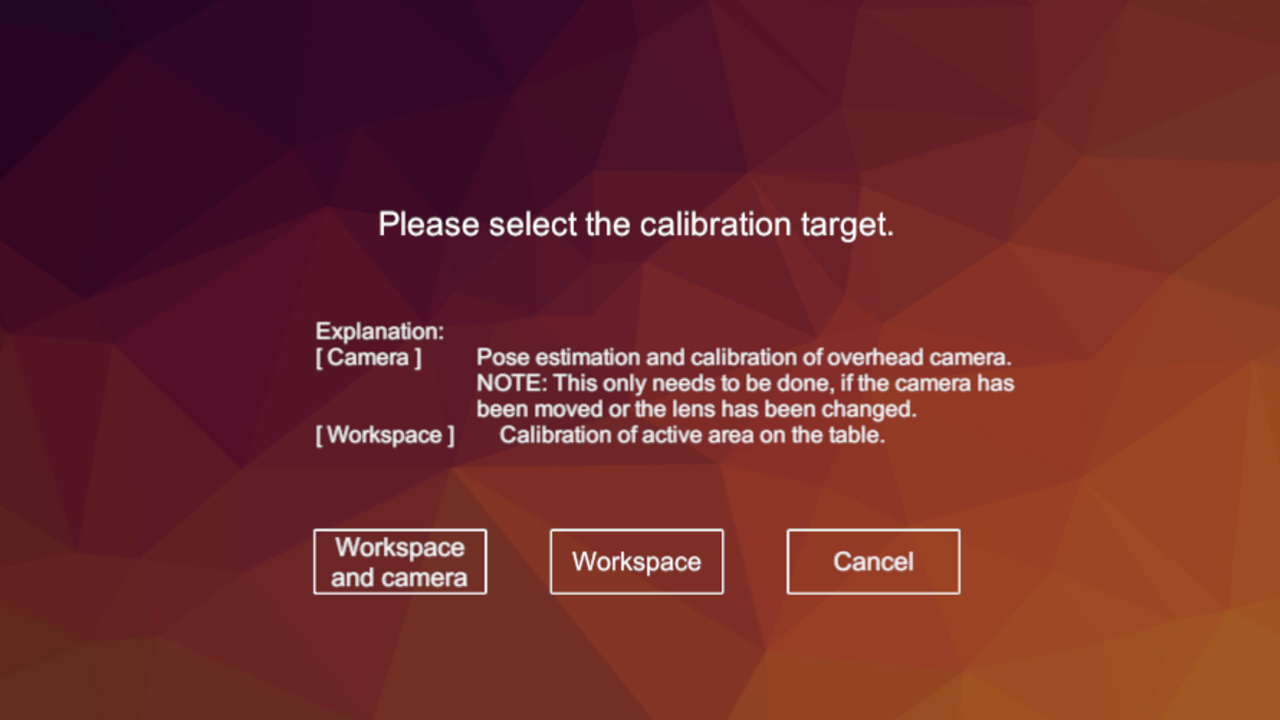
\includegraphics[trim=3cm 1cm 3cm 3cm, clip, width=0.9\textwidth]{Bilder/SelectCalibrationTarget.jpg}
			\label{fig:SelectCalibrationTarget}
	\end{figure}
\end{minipage}
\begin{minipage}{0.4\textwidth}
	\texttt{SelectCalibrationTarget}:\\
	Erlaubt die Auswahl der Art der Kalibrierung. Es kann hier entweder nur der Arbeitsbereich oder sowohl der Arbeitsbereich, als auch die Kamera kalibriert werden. Die Kalibrierung ist näher in \ref{sec:calib} beschrieben.
\end{minipage}\\

\begin{minipage}{0.6\textwidth}
	\begin{figure}[H] 
		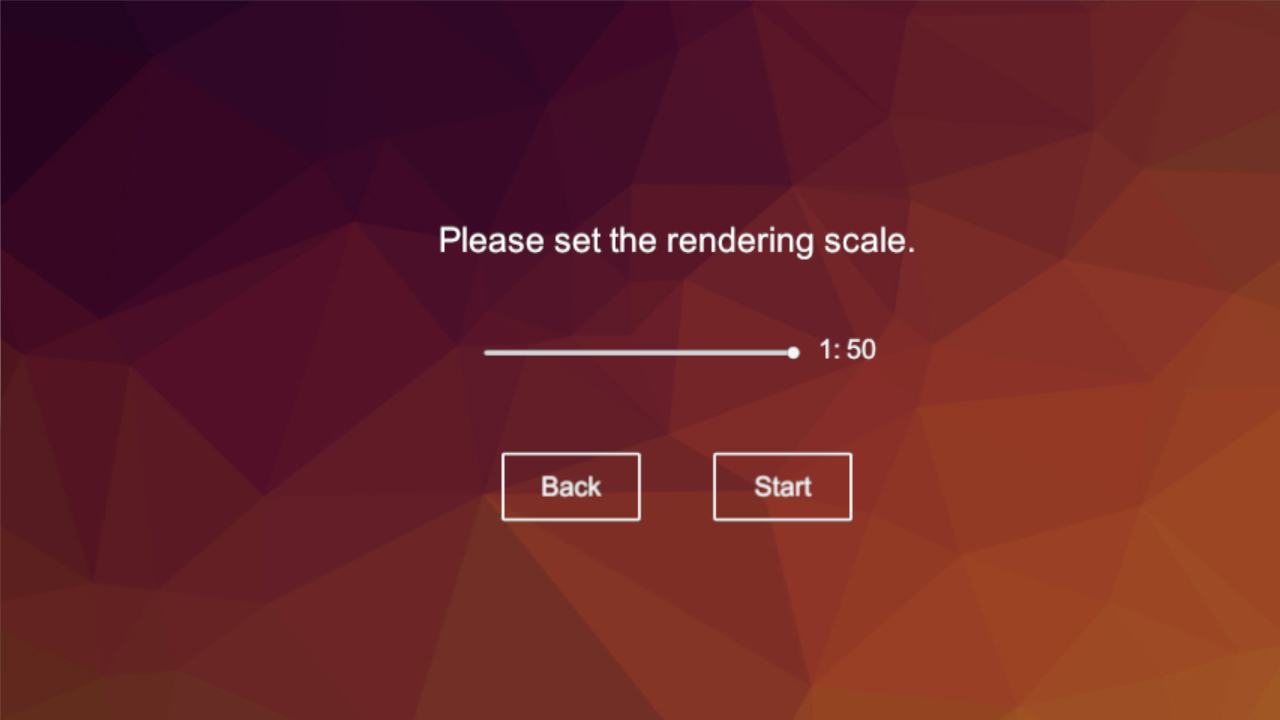
\includegraphics[trim=3.5cm 1cm 2.5cm 3cm, clip, width=0.9\textwidth]{Bilder/SetScale.jpg}
			\label{fig:SetScale}
	\end{figure}
\end{minipage}
\begin{minipage}{0.4\textwidth}
	\texttt{SetScale}:\\
	Stellt das letzte Menü vor dem Starten der Simulation dar. In diesem kann der Benutzer den Maßstab der Gebäudesimulation einstellen und anschließend die Simulation starten.
\end{minipage}\\

\begin{minipage}{0.6\textwidth}
	\begin{figure}[H] 
		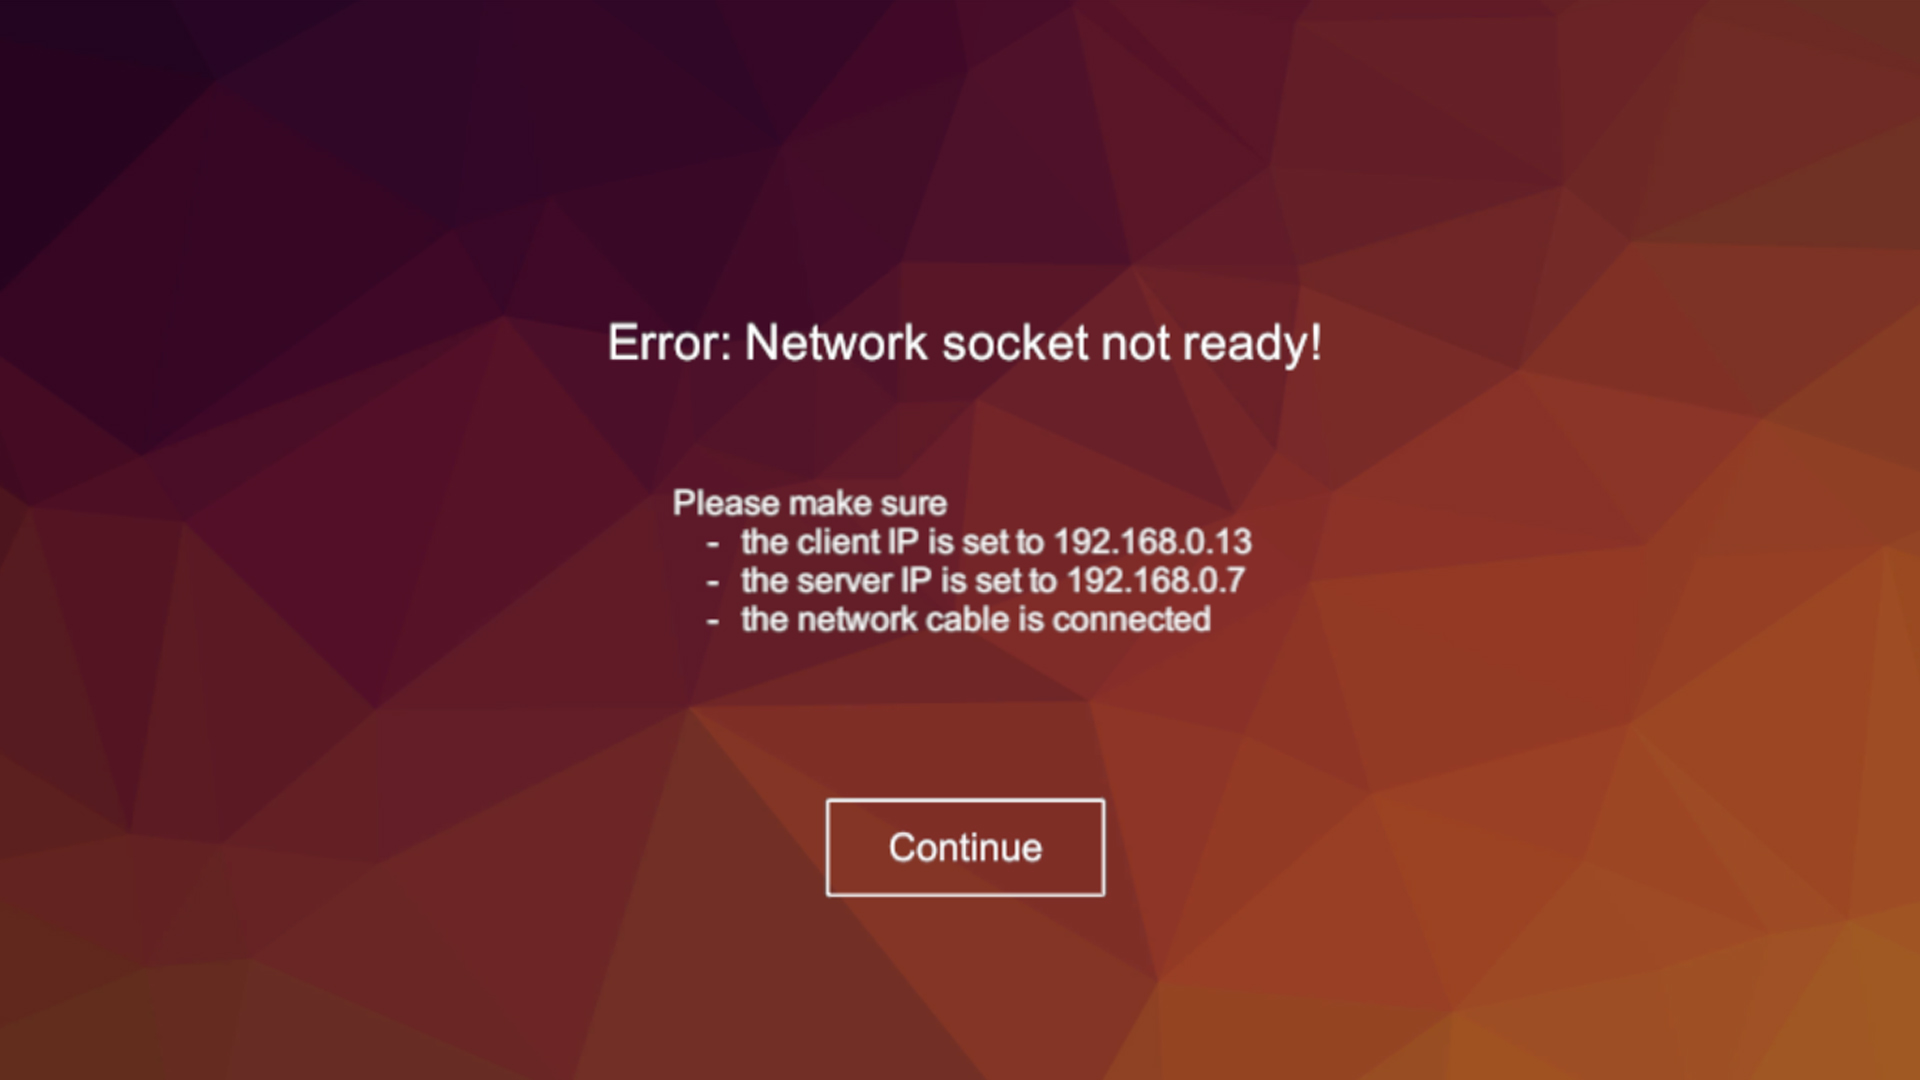
\includegraphics[trim=3cm 1cm 3cm 3cm, clip, width=0.9\textwidth]{Bilder/SocketNotReady.jpg}
			\label{fig:SocketNotReady}
	\end{figure}
\end{minipage}
\begin{minipage}{0.4\textwidth}
	\texttt{SocketNotReady}:\\
	Warnt den Benutzer nach dem Verlassen des \texttt{Welcome}-Menüs, dass die Netzwerkverbindung zwischen den beiden Computern nicht bereit ist. Nach Bestätigung dieses Hinweises durch einen Klick auf \texttt{Continue}, kehrt der Benutzer zum \texttt{Welcome}-Menü zurück. %Anschließend kann der Vorgang fortgesetzt werden, wenn die Netzwerkverbindung hergestellt wurde. Andernfalls erscheint wieder \texttt{SocketNotReady}.
\end{minipage}\\

\begin{minipage}{0.6\textwidth}
	\begin{figure}[H] 
		
\includegraphics[trim=3cm 2cm 3cm 2cm, clip, width=0.9\textwidth]{Bilder/Welcome.jpg}
			\label{fig:Welcome}
	\end{figure}
\end{minipage}
\begin{minipage}{0.4\textwidth}
	\texttt{Welcome}:\\
	Erscheint als erstes Menü. Hier erhält der Nutzer eine kurze Information darüber, wie die Anwendung heißt und wozu sie dient.
\end{minipage}\\

\subsubsection{Ablauf der Menüführung}\label{sec:menuAblauf}\todo[inline, color=green]{Lukas}
Der Ablauf der Menüführung von \textit{MArC} ist in Abbildung~\ref{fig:menuFlow} dargestellt. Die einzelnen Menüs sind bereits in~\ref{sec:menus} beschrieben worden.

\begin{figure}[htbp]
	\centering
	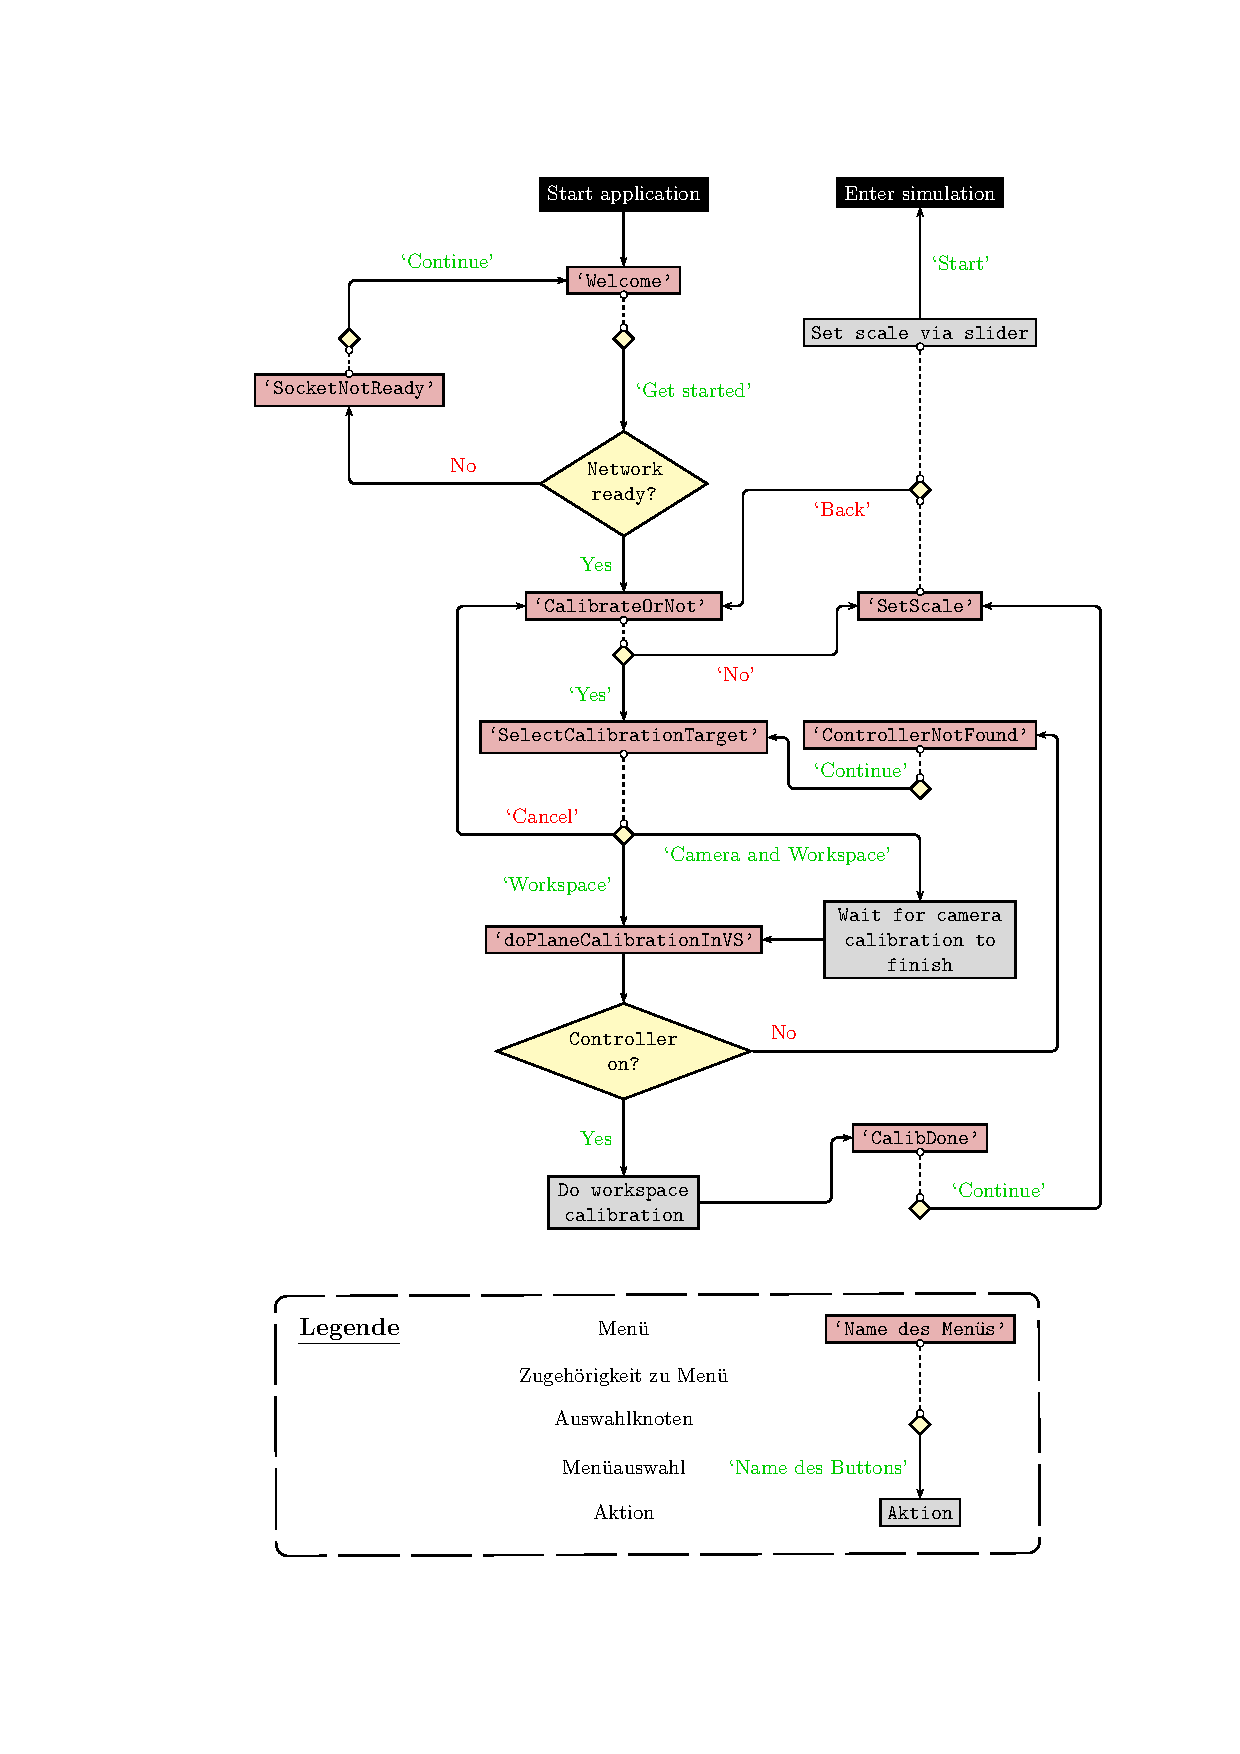
\includegraphics[scale=.9, trim=5.5cm 2.5cm 3.5cm 2.5cm]{kapitel/system/MP_Menu_Flowchart.pdf}
	\caption{Flussdiagramm der Menüführung.}
	\label{fig:menuFlow}
\end{figure}

Nach dem Starten der Anwendung wird zunächst das Menü \texttt{Welcome} angezeigt. Dieses enthält nur einen Button \textit{Get started}. Sobald dieser gedrückt wird, prüft die Anwendung, ob eine Netzwerkverbindung zu dem Computer mit der Tracking-Anwendung besteht. Sollte dies nicht der Fall sein, wird das Menü \texttt{Socket\-Not\-Ready} angezeigt. Dieses verlässt der Benutzer über einen Klick auf \texttt{Continue}, anschließend wird erneut das Menu \texttt{Welcome} angezeigt. Wenn zu diesem Zeitpunkt die Netzwerkverbindung korrekt hergestellt wurde, gelangt der Benutzer zum Menü \texttt{Calibrate\-Or\-Not}, anderenfalls wird wiederholt \texttt{Socket\-Not\-Ready} angezeigt.

In \texttt{CalibrateOrNot} hat der Benutzer die Auswahl zwischen den Schaltflächen \textit{Yes} und \textit{No}. Bei einem Klick auf \textit{Yes} wird anschließend \texttt{Select\-Calibration\-Target} angezeigt, bei einem Klick auf \textit{No} lädt das System eine zuvor durchgeführte Kalibrierung und das Menü \texttt{Set\-Scale} wird geöffnet.

\texttt{Select\-Calibration\-Target} stellt den Benutzer vor die Wahl entweder nur den Arbeitsbereich (\textit{Work\-space}) oder sowohl den Arbeitsbereich als auch die Kamera zu kalibrieren (\textit{Camera and Workspace}). Außerdem besteht die Möglichkeit über \textit{Cancel} zum Menü \texttt{Calibrate\-Or\-Not} zurückzukehren.

Wählt der Benutzer \textit{Camera and Workspace} in \texttt{Select\-Calibration\-Target} aus, so informiert die Anwendung die Tracking-Anwendung auf dem anderen Computer und wartet anschließend darauf, dass von dort die Bestätigung gesendet wird, dass die Kamerakalibrierung abgeschlossen ist. Anschließend wird das Menü \texttt{doPlane\-Calibration\-InVS} angezeigt, welches auch aufgerufen wird, wenn der Benutzer \textit{Work\-space} in \texttt{Select\-Calibration\-Target} wählt.

Im Menü \texttt{doPlane\-Calibration\-InVS} wird zunächst geprüft, ob der für die Kalibrierung notwendige HTC Vive Controller eingeschaltet ist. Sollte dies nicht der Fall sein, wird \texttt{Controller\-Not\-Found} aufgerufen. Dieses kann mit einem Klick auf \textit{Continue} verlassen werden, woraufhin wieder \texttt{Select\-Calibration\-Target} angezeigt wird.\\
Sofern der HTC Vive Controller beim Aufruf von \texttt{doPlane\-Calibration\-InVS} eingeschaltet ist, wird nach Durchführung der Kalibrierung des Arbeitsbereichs das Menü \texttt{CalibDone} angezeigt.

\texttt{Calib\-Done} kann über einen Klick auf \textit{Continue} verlassen werden und führt den Nutzer anschließend zu \texttt{SetScale}. Aus diesem Menü kann über den Button \textit{Back} entweder zu \texttt{CalibrateOrNot} zurückgekehrt oder die Simulation mit dem im Menü über den Slider eingestellten Maßstab gestartet werden.

\subsection{Toogle}\todo[inline]{Paul}

\subsection{Kontex Menü}\todo[inline]{Laura und Lukas}
\subsubsection{Menüführung}\todo[inline]{Laura}
\subsubsection{Architektur Berechnung}\todo[inline]{Laura}


\subsection{Table Menü}\todo[inline, color=yellow]{Paul}
\label{TableMenü}

Zur intuitiven Bedienung des \textit{MArC} wurden die Menüs, die während der Laufzeit benutzt werden können, auf dem Arbeitstisch platziert. Dies hat den Vorteil, dass zum einen diese Menüs permanent sichtbar sein können, ohne den Nutzer während der Arbeit zu stören und zum anderen ein haptisches Feedback bei der Nutzung möglich ist.\\
Möchte der Nutzer die Menüs bedienen, so drückt er mit dem Finger, der durch die \textit{Leap Motion} getrackt wird auf die Buttons und damit gleichzeitig auf den Tisch. Dies erleichtert die Benutzung deutlich im Vergleich zu der Nutzung von Menüs die im Raum schweben.\\
Im laufe der Entwicklung hat sich für das rechte Menü der Name \textit{Table Menü} etabliert. Im folgenden wird dessen Funktion im Detail erläutert.

\subsubsection{Szenen Management}\todo[inline, color=green]{Paul}
Eine Anforderung an das System war, dass der Nutzer erstellte Szenen abspeichern und wieder aufrufen können soll. Anhand des \textit{Table Menüs} ist dies möglich. Die Funktionen des Menüs sind:
\begin{itemize}
	\item Speichern von Szenen
	\item Laden von Szenen und aufrufen des \textit{Match Modus} (s. Abschnitt \ref{MatchModus})
	\item Scrollen durch die gespeicherten Szenen

\end{itemize}



\subsubsection{Speichern von Szenen}\todo[inline, color=green]{Paul}
\label{Speichern}
Möchte der Nutzer eine Szene speichern, so drückt er mit dem Finger auf den Button \glqq Save \grqq{}. \textit{MArC} speichert die aktuelle Szene automatisch in dem Ordner \glqq \textbackslash Resources\textbackslash saves\textbackslash Dateiname.xml\grqq{}.\\
Der Dateiame setzt sich aus aktuellem Datum und aktueller Zeit zum Speicherzeitpunkt wie folgt zusammen:
\begin{center}
	\texttt{Tag-Monat-Jahr-Stunde-Minute-Sekunde.xml}
\end{center}
Durch diese Markierung können später Dateien identifiziert werden, die auch nur Sekunden hintereinander gespeichert wurde.\\
Da innerhalb von \textit{Unity} eine hierarchiche Anordnung sämtlicher Elemente in Form eines Szenegraphen angewendet wird, bot sich eine Speicherung der Daten ebenfalls hierarchich in form eines XML Dokumentes an.\\
Die \textit{Extensible markup language (XML)} beschreibt eine Klasse von Daten Objekten (XML Documents) und ermöglicht das hierarchiche Abspeichern von geparsten oder ungeparsten Daten \cite{bray1998extensible}. In \textit{C\#} sind Verarbeitungsklassen bereits implementiert. Mittels dieser sog. \textit{XML Prozessoren} wird ein Datenzugriff erleichtert.

\paragraph{Dateiaufbau einer gespeicherten Szene}
Das gesamte Dokument wird mit einem Hauptknoten  \texttt{ $<$AR2\_COMPOSERSCENE$>$} umspannt. Innerhalb diesem wird mit texttt{ $<$time$>$}
ein Zeitstempel mit gespeichert, falls der Dateiname einmal umbenannt werden sollte.
Anschließend folgt der  texttt{ $<$TableObject$>$} Knoten, innerhalb dessen die Marker gespeichert werden. Jeder Marker wird nach dem folgenden Schema gespeichert, welches den Aufbau in Unity repräsentiert:


 \begin{lstlisting}
	<Name>
		<Kindknoten>
		<PositionX>
		<PositionY>
		<PositionZ>
		<RotationX>
		<RotationY>
		<RotationZ>
		<ScaleX>
		<ScaleY>
		<ScaleZ>
	</Name>
 \end{lstlisting}

Wobei sich dies als Kurzsschreibweise versteht, innerhalb der Positions/Rotations/Scale Knoten ist der entsprechende Wert eingetragen.

\paragraph{Vorgehen der Speicherung}
Das Skript \texttt{save.cs} ist für die Speicherung der Szenen verantwortlich. Zunächst wird der Zeitstempel geseichert und der Dateiname genertiert. Anschließend wird ein neues XML Dokument erstellt. An dieses wird zunächst der äußerste Knoten angehangen sowie der Zeitstempel. Anschließend wird die rekursive Funktion \texttt{traverseHierarchie} mit dem TableObject der Unity Szene aufgerufen und wird für jeden Kindknoten ausgeführt. \\
Diese Funktion erstellt jeweils die Knoten für den Namen, die Position, Rotation und Skalierung. Die Werte werden mittels \texttt{Node.InnerText} in die Knoten gespeichert.\\
Ist diese Funktion durch alle Kindknoten gegangen, wird am Ende noch die Skalierung der Szene in dem Knoten \texttt{globalBuildingScale} abgespeichert, damit dieser beim Laden der Szene rekonstruiert werden kann.

\subsubsection{Laden von Szenen}\todo[inline]{Paul}




\subsubsection{Match Modus}\todo[inline]{Paul}
\label{MatchModus}
\section{Tracking Programm} \label{sec:Tracking}\todo[inline]{Vera}
Zur Verfolgung und Positionsbestimmung der Würfel Marker (siehe Kapitel \ref{sec:WürfelMarker}) wurde ein Programm entwickelt, welche alle erforderlichen Resourcen und Funktionen bereit stellt und verknüpft. Zunächst muss die Initialisierung und der Zugriff der uEye Kamera (siehe Kapitel \ref{sec:uEye}) ermöglicht werden. Im Anschluss ist das Erstellen beziehungsweise laden aller relevanten Kalibrierungsinformationen unabdingbar. Nach erfolgreichem Abschluss beider Schritte führt das Programm  das Tracking der AruCo Marker und der grünen Rechtecke aus und steuert die Verwaltung und TCP Übertragung (siehe Kapitel \ref{sec:Netzwerk}) der Registrierten Würfel Marker Informationen. Diese Programm wurde in der IDE \textit{Visual Studio} (siehe Kapitel \ref{sec:VisualStudio}) in der Programmiersprache $C++$ entwickelt. Für die Entwicklungen wurden die uEye SDK, \textit{OpenCV} (siehe Kapitel \ref{sec:OpenCV}) sowie die Standardbibliothek \textit{Winsock} zur Hilfe genommen. In den folgenden Abschnitten wird die Vorgehensweise im Detail erklärt.

\subsection{uEye Ansteuerung}\todo[inline]{Vera}
Der erste Prozess des Tracking Programms ist die Initialisierung der uEye Kamera im Live-Bild-Modus. Mit Hilfe der vom Hersteller bereit gestellten SDK kann die Kamera mit allen benötigten Eigenschaften parametrisiert und alle notwendigen Speicher allokiert. Dies übernimmt die Funtion \texttt{inituEyeCam} in der Klasse \texttt{uEye\_input.cpp}. Die verwendeten Parameter können aus der Tabelle \ref{tab:UeyeParam} entnommen werden. Die Kamera wird mit dem maximalen Pixel Clock und der maximalen Framerate betrieben. Aus diesen Einstellungen ergibt sich auch die Belichtungszeit. Um einen höheren Kontrast zur Erkennung der Marker zu erzielen wurde zusätzlich das Hardware Signal zwanzigfach verstärkt.
Im Live-Bild-Modus werden die generierten Aufnahmen fortlaufend in der selben Speicheradresse überschrieben. Auf diesen Speicherplatz kann das Programm jederzeit mit der Funktion \texttt{getCapturedFrame} zugreifen, die die aktuellste Aufnahme zur Weiterverarbeitung zurück gibt. Nach der Beendigung des Tracking Algorithmus wird zusätzlich noch die Funktion \texttt{exitCamera} bereit gestellt, welche den verwendeten allokierten Speicher wieder freigibt.
\begin{table}
	\centering
	\begin{tabular}{|c|c|}
		\hline
		\Absatzbox{}
		\textbf{Parameter}& \textbf{Wert} \\
		\hline
		Pixel Clock & 37 ms \\
		\hline
		Frame Rate & 23 fps  \\
		\hline 
		Belichtungszeit & 40 ms\\
		\hline
		Gamma & 2.2 \\
		\hline
		Digitale Verstärkung & 20 \\
		\hline
	\end{tabular}
	\caption{Parametrisierung der uEye Kamera für das Tracking.}
	\label{tab:UeyeParam}
\end{table}

\subsection{Kalibrierung}\label{sec:calib}\todo[inline, backgroundcolor=green]{Laura}
Um das Ziel von \textit{MArC} zu erreichen, an den Positionen der Aluminiumwürfel im Arbeitsbereich in der virtuellen Realität von Unity gerenderte Würfel darzustellen, muss das System kalibriert werden. Die Kalibrierung hat zum Ziel, eine Koordinatentransformation zu finden, die Positionen im Kamera-Koordinatensystem in das Unity-Koordinatensystem transformiert.

Zu diesem Zweck muss eine zweistufige Kalibrierung durchgeführt werden. Zunächst sorgt die Kamerakalibrierung dafür, dass Bildkoordinaten auf dem Sensor der Kamera in das 3D-Kamera-Koordinatensystem transformiert werden. Dafür wird sich einiger OpenCV-Funktionen in Verbindung mit AruCo-Markern bedient. Dieser Vorgang wird nachfolgend in~\ref{sec:camCalib} genauer beschrieben.\\
Der nächste Schritt, die Kalibrierung des Arbeitsbereichs, bestimmt über Punkt-Korrespondenzen -- also in zwei verschiedenen Koordinatensystemen bekannte Punkte -- eine affine 3D-Transformation, welche die Abbildung vom Kamera-Koordinaten\-system auf das Unity-Koordinatensystem ermöglicht. Dieser Kalibrierungsschritt wird nachfolgend in~\ref{sec:planeCalib} näher beschrieben.\\
Trotz einer sorgfältigen Umsetzung der in den nächsten beiden Kapiteln beschriebenen Kalibrierungsschritte, ist es nicht gelungen, den Aluminiumwürfel und den gerenderten Würfel vollständig zur Deckung zu bringen. Der entstandene Fehler sowie mögliche systembedingte Fehlerquellen werden in~\ref{sec:calibError} und in~\ref{sec:calibErrorSources} beschrieben. 

\subsubsection{Kamerakalibrierung}\label{sec:camCalib}\todo[inline, backgroundcolor=green]{Laura}

Es gibt viele verschiedene wissenschaftliche Ausführungen über die Durchführung einer Kamerakalibrierung, wie z.B. \cite{5982395}, \cite{888718} und \cite{faugeras1993three}. Dabei unterscheidet man häufig zwischen automatischen und manuellen Kalibrierungen. \\
In Abbildung~\ref{fig:cameraCalib} sind die Zusammenhänge zwischen dem Projektionszentrumkoordinatensystem der Kamera, sowie deren Bildebene und dem Weltkoordinatensystem zu sehen. Im Gegensatz zu der Abbildung und den erwähnten Kalibrierungsansätzen reicht die Umrechnung von Bildkoordinaten in Weltkoordinaten, im vorliegenden Fall, nicht aus. Es muss eine Umrechnung der Bildkoordinaten in den Unity Raum erfolgen, um zu gewährleisten, dass die gerenderten Würfel anschließend deckungsgleich mit den Aluminiumwürfeln sind. Koordinaten des Unity Raumes werden im Folgenden Unitykoordinaten genannt.\\

\begin{figure}[H]
		\centering
		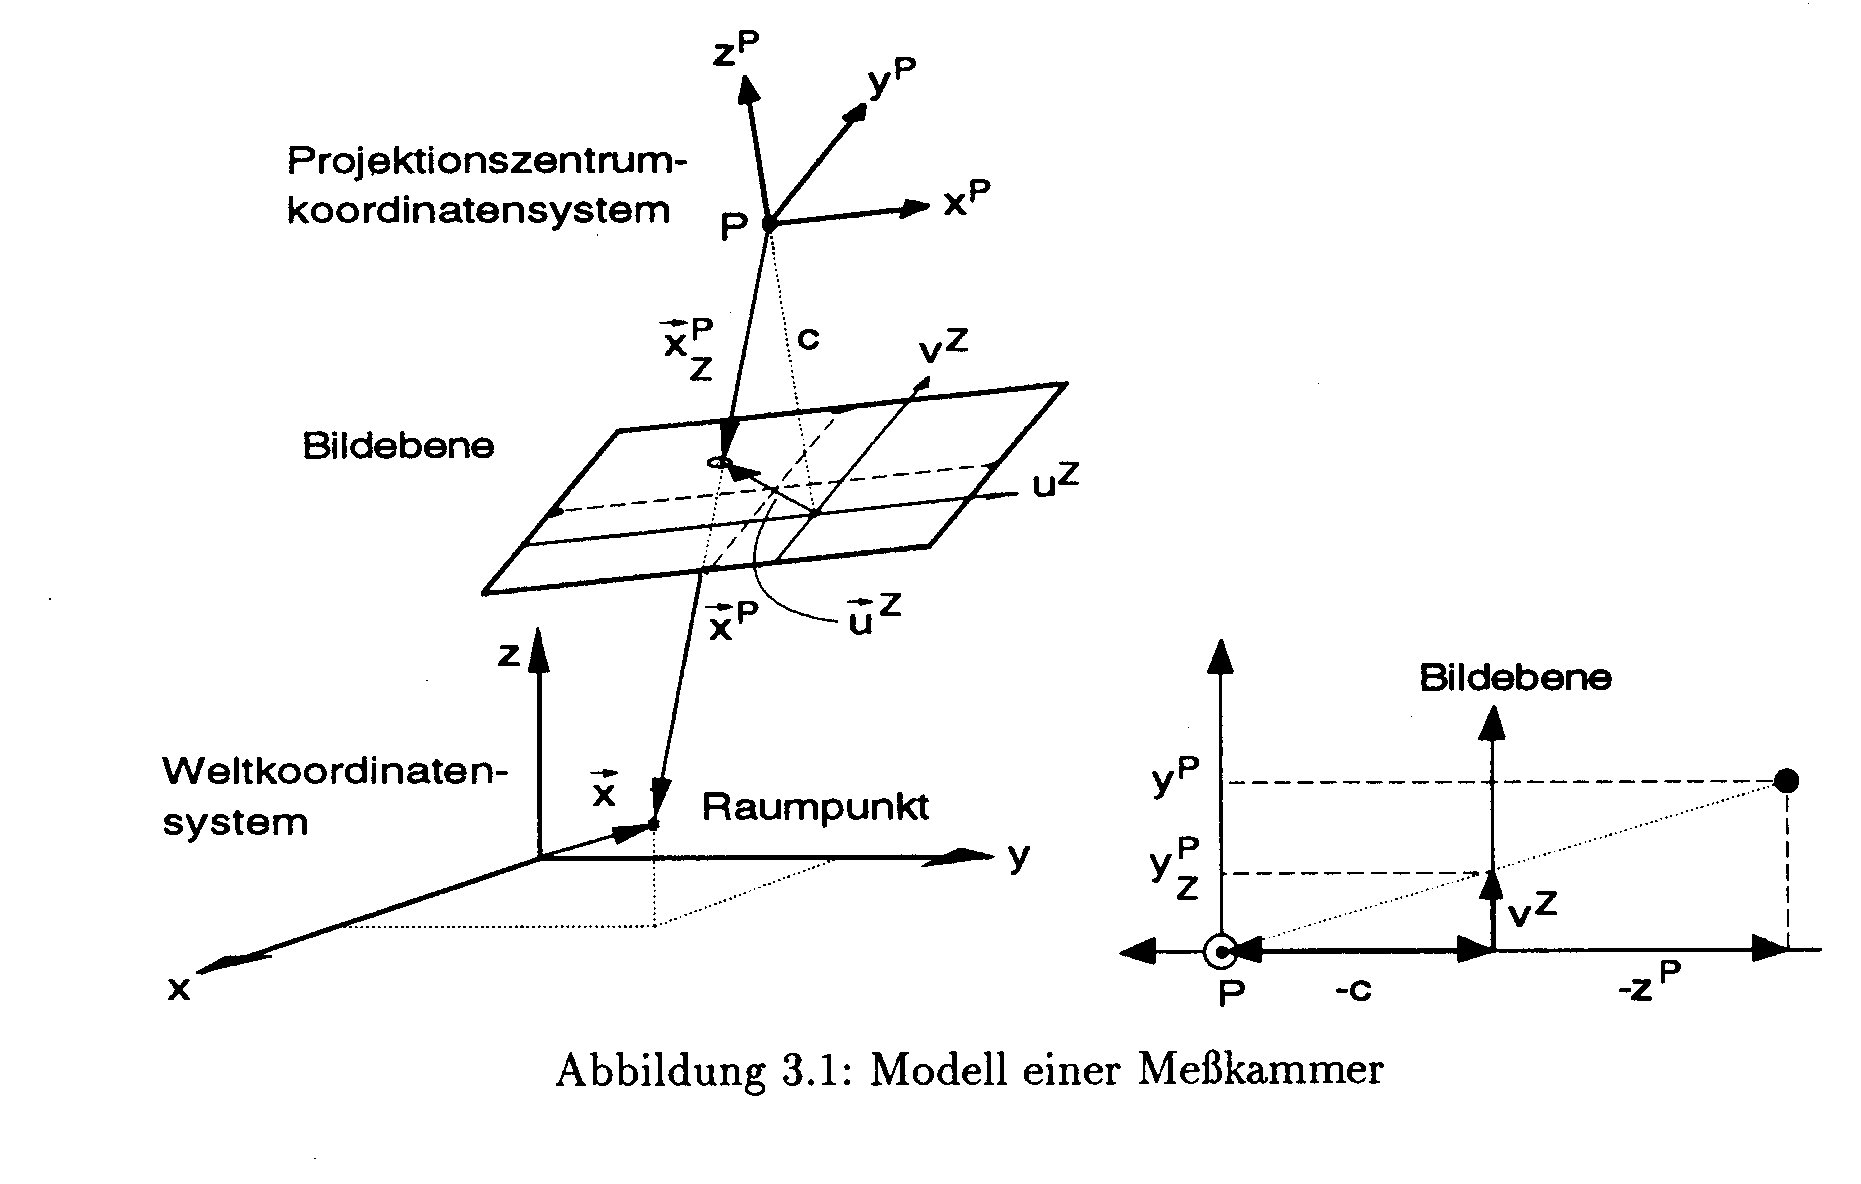
\includegraphics[width=0.65\textwidth , trim = 0mm 65mm 270mm 0mm, clip]{Bilder/cameraCalib.jpg}
			\caption{Lage des Kamerakoordinatensystems in Bezug auf Projektionsebene und Weltkoordinatensystem. \cite{Meisel:77890}}
			\label{fig:cameraCalib}
	\end{figure}

Die Kamerakalibrierung, die diesem Projekt zu Grunde liegt, ist als manuell einzustufen und kann, wenn gewünscht bzw. benötigt, zu Beginn der eigentlichen Anwendung durchgeführt werden. Um die verschiedenen Koordinatensysteme auseinander zu halten, wird zu Beginn eine Notation festgelegt, die in Tabelle~\ref{tab:camCalibParam} eingesehen werden kann. Zusätzlich können in der Tabelle sowohl die einzelnen Koordinatensysteme, als auch die einzelnen Berechnungsschritte der Kamerakalibrierung nachvollzogen werden, die im Folgenden erläutert werden. Lässt man die ersten zwei Zeilen der Tabelle weg, so ist eine Transformation von Weltkoordinaten $\overrightarrow{x}$ in Kamerakoordinaten $\overrightarrow{u}$ schematisch dargestellt. Dieses Schema muss für die Kamerkalibrierung von \textit{MaRC} invertiert werden und um die Koordinatentransformation in Unitykoordinaten ergänzt werden.  \\

\begin{table}
	\centering
	\renewcommand{\arraystretch}{1.4}
	\begin{tabular}{|c|c|c|c|}
		\hline
		\Absatzbox{}
		& \textbf{Koordinaten} & \textbf{Komponenten}&\textbf{Transformation}\\
		\hline
		$\overrightarrow{x}^U$ & Unity &$x^U$,$y^U$,$z^U$& \\
		\cline{2-4}
		$\downarrow$ & & & Koordinatentransformation\\
		\cline{2-4}
		$\overrightarrow{x}$ & Welt &$x$,$y$,$z$&  \\
		\cline{2-4}
		$\downarrow$ & & & Koordinatentransformation\\
		\cline{2-4}
		$\overrightarrow{x}^P$ & Projektionszentrum &$x^P$,$y^P$,$z^P$& \\
		\cline{2-4}
		$\downarrow$ & & & Projektion \\
		\cline{2-4}
		$\overrightarrow{x}^P_Z$ & Projektionszentrum &$u^Z$,$v^Z$,$-c$& \\
		\cline{2-4}
		$\downarrow$ & & & Linsenverzeichnung\\
		\cline{2-4}	
		$\overrightarrow{x}^P_D$ & Verzeichnung &$u^D$,$v^D$,$-c$& \\
		\cline{2-4}
		$\downarrow$ & & & Bildebenenverkippung\\
		\cline{2-4}		
		$\overrightarrow{x}^V$ &Verkippung &$u^V$,$v^V$,$-c^V$& \\
		\cline{2-4}
		$\downarrow$ & & & Bildhauptpunktverschiebung\\
		\cline{2-4}	
		$\overrightarrow{u}$ & Sensor &$u$,$v$ & \\
		\hline
	\end{tabular}
	\caption{Parameter und Berechnungsschritte der Kamera Kalibrierung.\cite{Meisel:77890}}
	\label{tab:camCalibParam}
\end{table}

Die einzelnen Schritte aus Tabelle~\ref{tab:camCalibParam} kann man in vier bzw. drei Abschnitte einteilen: \\
Im ersten Abschnitt wird der Hauptpunkt so versetzt, dass der Koordinatenursprung des Kamerakoordinatensystems mit dem Bildkoordinatensystem übereinstimmt. Dies geschieht, indem man für die eine Achse $u^V = u - \Delta u$ und für die andere Achse entsprechend $v^V = v - \Delta v$ berechnet.\\
Zusätzlich wird die Bildebene verkippt, so dass gilt $\overrightarrow{x}^V = R_v \cdot \overrightarrow{x}^P_D$. Bezeichnet $\varphi$ den Drehwinkel um die $x^P$-Achse und $\vartheta$ den Drehwinkel um die $y^{P'}$-Achse, so lässt sich $R_v$ wie folgt berechnen:

\begin{equation}
\label{equ:Rverkippt}
R_v = 
\begin{pmatrix}
r_{v11} & r_{v12} & r_{v13} \\
r_{v21} & r_{v22} & r_{v23} \\
r_{v31} & r_{v32} & r_{v33} \\
\end{pmatrix} = 
\begin{pmatrix}
cos\vartheta & sin\vartheta sin\varphi & -sin\vartheta cos\varphi \\
0 & cos\varphi & sin\varphi\\
sin\vartheta & -cos\vartheta sin\varphi & cos\vartheta cos\varphi \\
\end{pmatrix} 
~ ~ ~ ~ ~R_v \in \mathbb{R}^{3x3}
\end{equation}

Die negative verkippte Kamerakonstante $-c^V$, die in Tabelle~\ref{tab:camCalibParam} aufgeführt ist, berechnet sich wie in~\citep{Meisel:77890} beschrieben nach der Formel:

\begin{equation}
-c^V = - \frac{c+u^V \cdot r_{v13} + v^V \cdot r_{v23}}{r_{v33}}
\end{equation}

Im zweiten Schritt wird im Allgemeinem die Linsenverzeichnung herausgerechnet. Im vorliegenden Fall wurde bewusst auf diesen Schritt verzichtet und die zugehörigen Entzerrungskoeffizienten werden für alle weiteren Berechnungen auf null gesetzt. Dieses Vorgehen wurde gewählt, da einige Tests gezeigt haben, dass die berechneten Entzerrungskoeffizienten stark voneinander abgewichen sind, obwohl dies beim Benutzen der gleichen Kameraeinstellungen und dem gleichen Objektiv nicht der Fall sein dürfte.\\
Weil wie bereits beschrieben, die Linsenverzeichnung vernachlässigt wurde, kann man Schritt 1 und 2 zu einem Schritt zusammenfassen und vereinfacht darstellen. Dieser erste Schritt, also die Hauptpunktverschiebung und Bildebenenverkippung, lässt sich mit Hilfe der intrinsischen Kameramatrix $M_{intrinsisch}$ zusammenfassen. Diese beinhaltet neben den Brennweiten $f_u$ und $f_v$ noch die Koordinaten des Hauptpunktes $u^V$ und $v^V$ in Bildkoordinaten und hat somit vier Freiheitsgrade.

\begin{equation}
\label{equ:intrinsic}
M_{intrinsisch} = 
\begin{pmatrix}
f_u & 0 & 0 & u^V \\
0 & f_v & 0 & v^V\\
0 & 0 & 1 & 0 \\
\end{pmatrix} 
~ ~ ~ ~ ~M_{intrinsisch} \in \mathbb{R}^{3x4}
\end{equation}

Zu diesem Zeitpunkt sollte nun das Kamerakoordinatensystem mit dem Weltkoordinatensystem übereinstimmen und es kann sich im nächsten Schritt darum gekümmert werden, dass das Kamerakoordinatensystem verschoben und gedreht wird. Während eine dreidimensionale Rotation im Allgemeinen mit Matrix $R$ aus Formel~\ref{equ:Rotation} beschrieben werden kann, reicht für die Translation ein Vektor, wie $t$ aus Formel~\ref{equ:Translation} aus.\

\begin{equation}
\label{equ:Rotation}
R= R_\gamma ~R_\beta ~R_\alpha =
\begin{pmatrix}
r_{11} & r_{12} & r_{13} \\
r_{21} & r_{22} & r_{23} \\
r_{31} & r_{32} & r_{33} \\
\end{pmatrix}
~ ~ ~ ~ ~R \in \mathbb{R}^{3x3}
\end{equation}



\begin{equation}
\label{equ:Translation}
t=
\begin{pmatrix}
t_x & t_y & t_z
\end{pmatrix}^T
~ ~ ~ ~ ~t \in \mathbb{R}^{3x1} 
\end{equation}

Diese beiden Transformationen können wie in Formel~\ref{equ:extrinsic} zur extrinsischen Kameramatrix $M_{etrinsisch}$ zusammengefasst werden. Diese hat sechs Freiheitsgrade, nämlich drei für den Translationsvektor $t$ und drei für die Eulerwinkel der Rotationsmatrix $R$ für die dementsprechend gelten muss $R \in SO(3)$.

\begin{equation}
\label{equ:extrinsic}
M_{extrinsisch}= 
\begin{pmatrix}
R &|& t \\
\end{pmatrix} 
~ ~ ~ ~ ~M_{extrinsisch} \in \mathbb{R}^{3x4}
\end{equation}

Schritt 1 und 2 lassen sich vereinfachen, indem man die intrinsische Kameramatrix $M_{intrinsisch}$ und die extrinsische Kameramatrix $M_{extrinisch}$ nach der Formel~\ref{equ:inAndEx} zu einer Matrix $M$ zusammenfasst.

\begin{equation}
\label{equ:inAndEx}
M = M_{intrinsisch} \cdot M_{extrinsisch}~ ~ ~ ~ ~M\in \mathbb{R}^{3x4}
\end{equation}

Die Umrechnung von Kamerakoordinaten in Weltkoordinaten kann dann mit der invertierten Matrix $M$, wie in Formel~\ref{equ:SensInWorld} berechnet werden. \

\begin{equation}
\label{equ:SensInWorld}
\overrightarrow{x} = M^{-1} \cdot \overrightarrow{u}
\end{equation}

An diesem Punkt hat man die Kamerakoordinaten vollständig in Weltkoordinaten überführt und sucht nun eine Transformationsmatrix um diese Punkte auf ihre korrespondierenden Punkte in Unitykoordinaten abzubilden. Die dazu benötigte affine 3D-Transformation wird in Kapitel \ref{sec:planeCalib} erläutert.


\subsubsection{Kalibrierung des Arbeitsbereichs}\label{sec:planeCalib} \todo[inline]{Laura}

%Entsprechend Formel~\ref{equ:SensInWorld} muss für den letzten Schritt eine Transformationsmatrix von Weltkoordinaten in Unitykoordinaten gefunden werden. Dies geschieht indem man die korrespondierenden Koordinatenpaare einer Controllerposition in Unity und in bereits in Weltkoordinaten gebrachten Sensorkoordinaten ineinander überführt, d.h. eine affine Transformation durchführt. Die Controlerpositionen in Weltkoordinaten werden somit auf die in Unitykoordinaten abgebildet.
\subsubsection{Kalibrierungfehler} \label{sec:calibError}\todo[inline]{Laura}
\subsubsection{Mögliche Fehlerquellen} \label{sec:calibErrorSources}\todo[inline]{Laura}

\subsection{Marker Detektion}
\subsection{Green Keying}\todo[inline]{Vera}
\subsection{ArUco Marker Tracking}\todo[inline]{Vera}

\subsection{Marker Objekt}\todo[inline]{Vera}
\subsection{Zuordnung der Identitäten}\todo[inline]{Vera}


\section{Auswertung}
\subsection{Testing durch unerfahrene Benutzer}
\subsection{Testing durch Architekten}

\section{Zusammenfassung}\todo[inline, color=green]{Lukas}
\todo[inline, color=blue]{Paul}
In der vorliegenden Dokumentation wurde \emph{MArC}, der "`Mixed Reality Architecture Composer"' vorgestellt und detailliert beschrieben.\\
Zunächst erfolgte dazu in Kapitel~\ref{sec:Einleitung} die Einordnung des Projektvorhabens in die Ziel-Umgebung, außerdem wurde das Ziel des Projekts erläutert. Das Produkt \emph{MArC} sollte ein Werkzeug sein, welches Architekten die frühe Entwicklung von Siedlungen erleichtert. Auf architektonische Details der einzelnen Gebäude wurde dabei bewusst verzichtet, da \emph{MArC} vor allem bei der Platzierung der Gebäude behilflich sein soll.\\
In Kapitel~\ref{sec:grundlagen} wurden Grundlagen erörtert, die für die nachfolgenden Teile der Dokumentation für den Leser relevant sind. Diese Grundlagen beinhalten Theorie für die Entwicklung von Virtual-Reality-Anwendungen und damit verbundene Interaktionsmethoden, den grundlegenden Aufbau von Netz\-werk-Kom\-mu\-ni\-ka\-tions\-systemen, sowie eine Einführung in markerbasierte Objektverfolgung.\\
Alle während des Projekts verwendeten und erstellten Ressourcen, insbesondere Hard- und Software, wurden im Detail in Kapitel~\ref{sec:Materialien} thematisiert. Auch die in der ursprünglichen Projektplanung vorgesehene, später aber doch nicht verwendete Hardware wird dort beschrieben.\\
In Kapitel~\ref{sec:system} wurde das während der Projektlaufzeit entwickelte System vorgestellt. Neben dem grundsätzlichen Aufbau und der Verwendung des Systems durch einen Benutzer wurden auch die Netz\-werk-Kom\-mu\-ni\-ka\-tion der beiden Haupt-Soft\-ware\-kom\-po\-nen\-ten, die Menüführung vor dem Starten der \emph{Unity}-Simulation, sowie die Interaktion mit dem System als VR-Anwendung beschrieben.\\
Dem Tracking Programm als einem der Hauptteile von \emph{MArC} wurde das Kapitel~\ref{sec:Tracking} gewidmet. Darin wird sowohl die Anbindung der Kamera über dem Arbeitsbereich an die Tracking-Anwendung beschrieben, als auch die Kalibrierung des Systems mit den Koordinatentransformationen thematisiert, die nötig sind, um die Positionen der Würfel-Marker in den Koordinatenraum der \emph{Unity}-Simulation zu überführen. Des weiteren wird der Umgang der Tracking-Anwendung mit der Detektion, Verfolgung und Registrierung der verwendeten Marker behandelt.\\
In Kapitel~\ref{sec:ausblick} wurde ein kurzer Ausblick darüber gegeben, welche dem Projekt folgenden, weiteren Entwicklungsmaßnahmen von \emph{MArC} das Projektteam als sinnvoll erachtet. Dies beinhaltet neben Verbesserungen des verwendeten Marker-Tracking-Systems eine Erweiterung von \emph{MArC} mit einer auf dem Head-Mounted-Display montierten Kamera zu einer Augmented-Reality-Anwendung, wie sie zu Beginn dieses Projekts geplant war. Im Ausblick wird zusätzlich der Im- und Export von 3D-Modell-Daten für die Interoperabilität von \emph{MArC} mit Modellierungs- und Entwicklungssoftware behandelt, welche in Architekturbüros Anwendung findet. Außerdem wird eine Studie zur Gebrauchstauglichkeit von \emph{MArC} empfohlen, um insbesondere die Interaktionsmethoden der VR-Anwendung daraufhin zu überprüfen, ob diese tatsächlich zu einer gesteigerten Effizienz für Architekten bei der Siedlungsentwicklung führen.\\
Mit dem Projektmanagement, welches bei einem Masterprojekt wie \emph{MArC} eine zentrale Rolle spielt, befasst sich das Kapitel~\ref{sec:pm}. Dort wird die zu Beginn des Projekts erarbeitete Projektdefinition ebenso thematisiert wie die Projektplanung mit Arbeitspaketen, Meilensteinen und verschiedenen Plänen, die helfen sollen, die Planung und den Fortschritt des Projekts zu quantifizieren. Der Durchführung des Projekts mit dem Fokus auf der Zusammenarbeit im Projektteam und dem Projektabschluss sind ebenfalls Abschnitte gewidmet. Als weiteren wichtigen Teil der Analyse des Projekts ist die Reflexion in Abschnitt~\ref{sec:reflexion} anzusehen. Da die Erwartungen an das Projekt \emph{MArC} mehrfach während der Projektdauer angepasst und gesenkt werden mussten, weil viele unerwartete~--~und teils selbst verschuldete~--~Probleme auftraten, war es im Interesse des Projektteams, das Projekt besonders im Hinblick auf diese Schwierigkeiten kritisch zu analysieren und diese Reflexion in die Dokumentation mit einfließen zu lassen.

\section{Steckbrief}\todo[inline]{Vera} \todo[inline, color=blue]{Paul}


\newpage
\bibliographystyle{plain}
\bibliography{main}
\end{document}